\documentclass[11pt]{article}
\usepackage[review]{acl}
\usepackage{times}
\usepackage{latexsym}
\usepackage[T1]{fontenc}
\usepackage[utf8]{inputenc}
\usepackage{microtype}
\usepackage{hyperref}
\usepackage{url}
\usepackage{booktabs}
\usepackage{amsmath}
\usepackage{amssymb}
\usepackage{graphicx}
\usepackage{makecell}
\usepackage{xcolor}
\usepackage{enumitem}
\usepackage{placeins}

\setlength\titlebox{6.2cm}
\setlength{\textfloatsep}{7pt plus 1pt minus 2pt}
\setlength{\floatsep}{6pt plus 1pt minus 2pt}
\setlength{\intextsep}{6pt plus 1pt minus 2pt}
\setlist[itemize]{leftmargin=1.15em,topsep=2pt,itemsep=1pt,parsep=0pt}

\newcommand{\method}{\textsc{INSIGHT}}
\newcommand{\cbm}{\textsc{CBM}}
\newcommand{\caac}{\textsc{CAAC}}
\newcommand{\cgta}{\textsc{CGTA}}
\newcommand{\crs}{\textsc{CRS}}
\newcommand{\tsd}{\textsc{TSD}}

\title{\method: A Language-Grounded Risk Concept Interface for Interpretable Accident Anticipation}
\author{Anonymous Submission}

\begin{document}
\maketitle

\begin{abstract}
Accident anticipation is usually optimized as an opaque binary prediction task.
For safety-critical use, a strong score is not enough: the model should expose
what it treats as risky and how those semantics affect warning behavior. We
present \method{}, an interpretable anticipation framework built around a
governed language-grounded risk concept interface. The interface mines
candidate concepts from driving frames, canonicalizes them into reusable risk
primitives, balances semantic families, and exports a trainable ontology with
review metadata and merge provenance. The ontology becomes the concept
bottleneck of an anticipation model, making semantic-interface design a
measurable modeling choice. Across DAD and A3D, \method{} reaches a compact
interpretable operating point, including 93.40\% AP and 4.90s mTTA on A3D and
68.19\% AP on the canonical DAD curriculum line with about 30M parameters.
The strongest claim is methodological: ontology construction is not hidden
preprocessing, but a governed semantic interface whose downstream effects can
be evaluated.
\end{abstract}

\section{Introduction}

Useful accident anticipation systems should do more than emit a final risk
score. In ADAS and autonomous-driving pipelines, an operator or auditor needs a
stable intermediate object: a semantic layer that names the hazards being used,
lets alternative vocabularies be compared, and reveals how semantics affect the
accuracy--timeliness operating point. Current systems rarely provide this
object. Strong anticipation models improve AP and warning time with recurrent,
graph, attention, or multimodal architectures~\citep{ref4,ref17,liao2024crash},
while explanation-oriented systems often add post-hoc visualization or
language after prediction~\citep{ref2,liao2024and}. These tools are useful, but
they do not make the semantic vocabulary itself a trainable and auditable part
of the model.

\begin{figure*}[t]
  \centering
  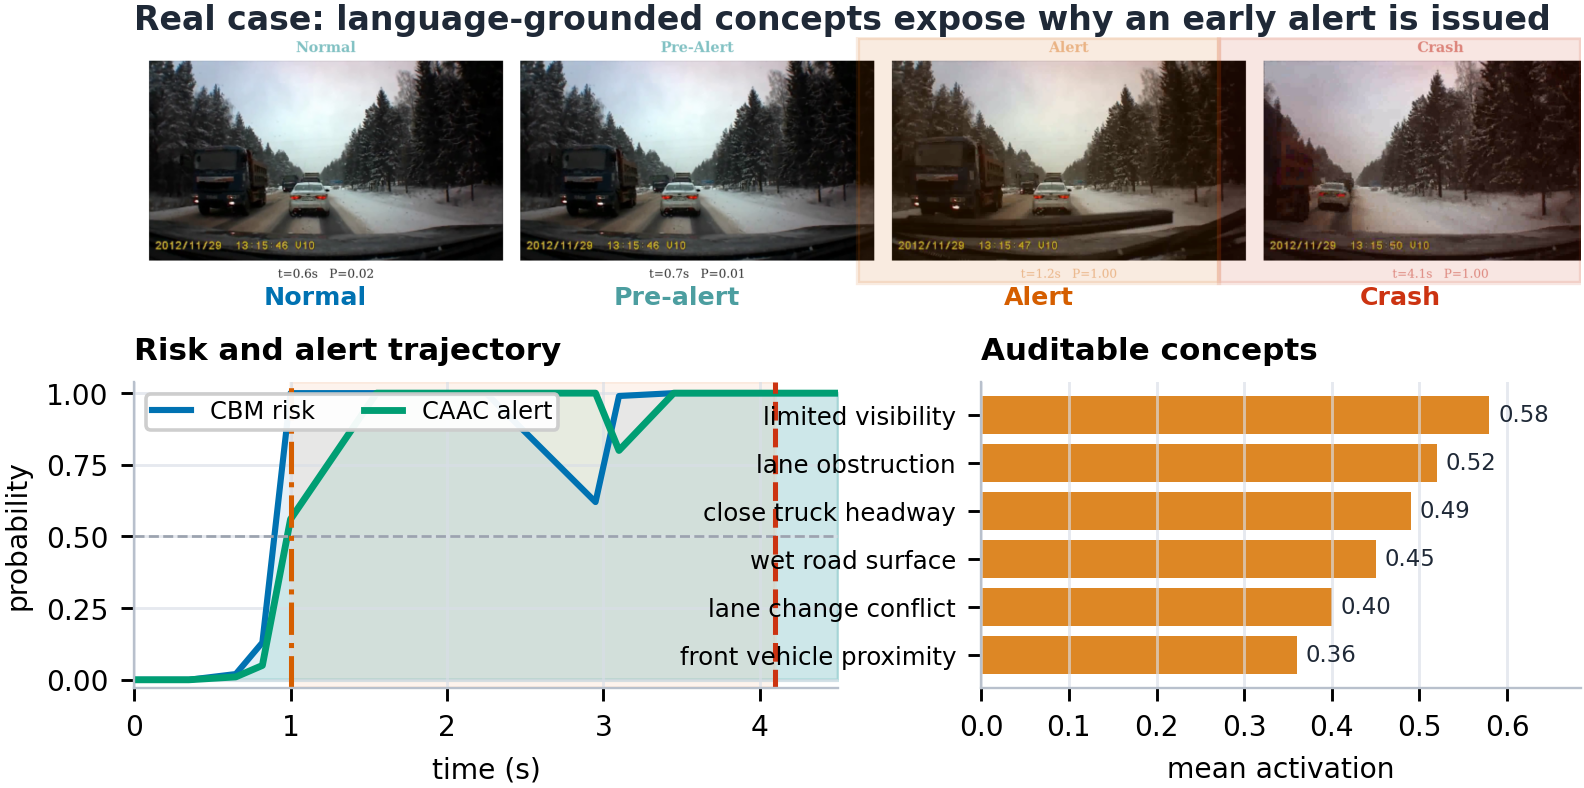
\includegraphics[width=0.98\textwidth]{../figures/emnlp_fig1_case_interface.pdf}
  \caption{\textbf{Semantic interface in action.} A real crash sequence is
  paired with a compact risk trajectory and named concept activations. The
  figure is a motivated example: quantitative claims remain tied to the
  protocol-separated tables.}
  \label{fig:case}
  \label{fig:motivation}
\end{figure*}

We argue that the missing object is a \emph{language-grounded risk concept
interface}. The interface is not a prompt artifact or a figure decoration. It
is a governed ontology that becomes the model's semantic bottleneck and can
therefore be changed, audited, and evaluated. Figure~\ref{fig:case} shows the
desired reader experience: named concepts, temporal evidence, and warning
behavior are visible together before any leaderboard discussion.

Our contributions are:
\begin{itemize}
  \item We formulate accident anticipation around a governed semantic interface,
  treating ontology construction as a modeling choice rather than hidden
  preprocessing.
  \item We introduce a reproducible concept-construction pipeline that mines,
  refines, merges, balances, and lightly reviews risk concepts into a trainable
  ontology.
  \item We build \method{}, a compact concept-bottleneck anticipation model
  that exposes concept-level risk evidence while preserving competitive
  predictive utility.
  \item We show that ontology choice changes the AP--mTTA operating point under
  matched launchers on DAD and A3D. DAD fragility and actor-policy timing are
  kept as scoped support evidence.
\end{itemize}

\section{Related Work}

\paragraph{Accident anticipation.}
Accident anticipation methods model pre-crash video prefixes to predict whether
an accident will occur, often optimizing AP and time-to-accident metrics
\citep{ref4,ref17,liao2024crash}. Recent systems such as CCAF-Net
\citep{liu2025ccaf} and LATTE~\citep{ZHANG2025103173} improve DAD scores, but
they do not expose a trainable semantic state that can be named, varied, and
audited across runs.

\paragraph{Language grounding and interpretability.}
Post-hoc visual explanations localize evidence after a prediction, and
language-based systems can verbalize accident regions or scene descriptions
\citep{ref2,liao2024and}. \method{} instead places language-derived risk
concepts inside the forward path. It is related to concept bottlenecks and
interpretable representation learning~\citep{tishby2000information}, but the
vocabulary itself is governed and experimentally varied in the accident
anticipation setting.

\section{Method}

\begin{figure*}[t]
  \centering
  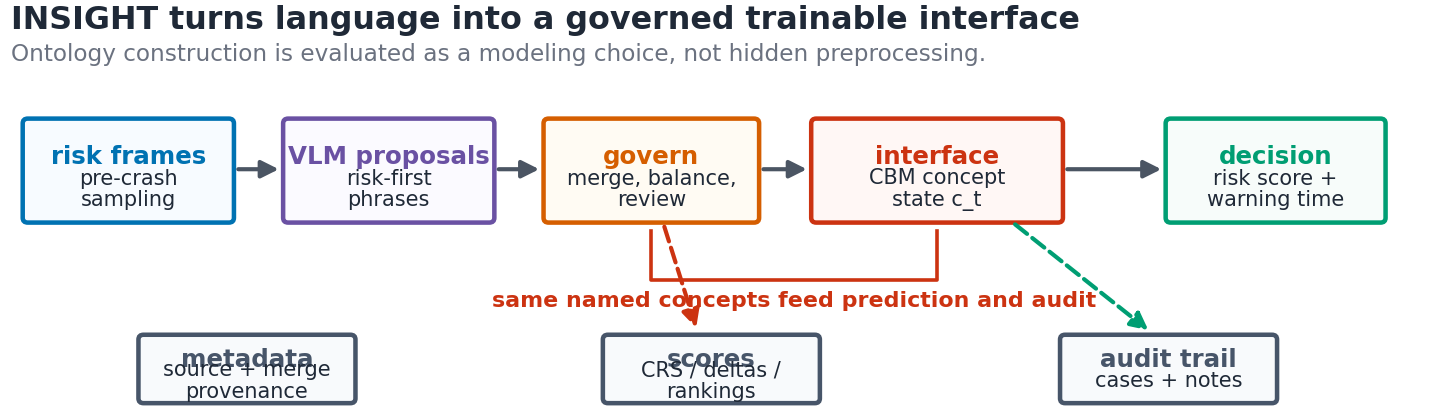
\includegraphics[width=0.98\textwidth]{../figures/emnlp_fig2_pipeline.pdf}
  \caption{\textbf{\method{} centers the language-grounded semantic interface.}
  The same named concepts support prediction, risk scoring, and audit outputs;
  ontology construction is therefore part of the method, not a hidden data
  cleaning step.}
  \label{fig:pipeline}
\end{figure*}

Given a dashcam video $\{\mathbf{x}_t\}_{t=1}^T$, accident label $y$, and
accident time $\tau$, standard anticipation predicts whether an accident will
occur from a prefix. We instead optimize for a useful operating region:
predictive quality with warning lead time and an inspectable semantic state,
\begin{equation}
  \max_{\theta}\; \mathbb{E}[\mathrm{TTA}]
  \quad \mathrm{s.t.}\quad
  \mathrm{AP}(\theta)\geq \mathrm{AP}_{\text{base}}.
\end{equation}
The key design variable is the semantic interface used to represent risk.

\paragraph{Governed ontology construction.}
The vocabulary is built in five stages. We sample diverse pre-crash frames,
ask a multimodal model for risk-first concepts rather than generic captions,
canonicalize noisy proposals into reusable primitives, balance semantic
families, and export a paper-facing ontology with names, family tags, merge
provenance, and review notes. This makes the ontology reproducible enough to
compare against compact manual and large historical vocabularies.

\paragraph{Concept-bottleneck anticipation.}
Once an ontology is fixed, \method{} maps object-focused frame features
$\mathbf{o}_t$ to concept activations $\mathbf{c}_t\in[0,1]^K$:
\begin{equation}
\begin{aligned}
  \mathbf{c}_t &= \sigma(\mathbf{W}_c\mathbf{o}_t+\mathbf{b}_c),\\
  \mathbf{e}_t &= \mathrm{LayerNorm}(\mathbf{W}_d\mathbf{c}_t+\mathbf{b}_d).
\end{aligned}
\end{equation}
The bottleneck is supervised with CLIP-derived top-$m$ pseudo-labels
($m=3$ in the main recipe), treated as semantic bootstrapping rather than dense
human frame-level ground truth. We compute a global concept risk score
$\rho_t=\sigma(\mathbf{w}_{\mathrm{risk}})^\top\mathbf{c}_t$, use \cgta{} to
focus history on semantic changes, and use \tsd{} to distill future CLIP
features into current representations. \caac{} consumes the concept-augmented
state for timing; in this paper actor timing remains support evidence rather
than the central causal claim.

\section{Experiments}

\paragraph{Setup and evidence discipline.}
We evaluate on DAD~\citep{ref4} and A3D~\citep{liao2024crash}. DAD is a
fragile stress setting with short-horizon transitions. A3D is the cleaner
flagship setting where precursor concepts appear earlier. Models use VGG16 ROI
features~\citep{ref31}, AdamW, and matched launcher families. We separate
headline runs, controlled ontology comparisons, and stress diagnostics instead
of pooling heterogeneous checkpoints into one leaderboard narrative.

\begin{table*}[t]
\centering\small
\setlength{\tabcolsep}{4pt}
\caption{\textbf{Headline predictive evidence.} DAD is reported as a stress
setting; A3D is the cleaner flagship result. \method{} is positioned as a
compact semantic-interface model rather than an unrestricted leaderboard
claim.}
\label{tab:headline_polished}
\label{tab:dad}
\label{tab:a3d}
\begin{tabular}{llccccc}
\toprule
Data & Method & AP$\uparrow$ & mTTA$\uparrow$ & TTA@R80$\uparrow$ & P@R80$\uparrow$ & Interface \\
\midrule
DAD & DRIVE~\citep{ref2} & 58.4\% & 2.31s & -- & -- & post-hoc \\
DAD & CRASH~\citep{liao2024crash} & 65.3\% & 1.75s & -- & -- & none \\
DAD & CCAF-Net~\citep{liu2025ccaf} & 81.3\% & 4.15s & -- & -- & none \\
DAD & LATTE~\citep{ZHANG2025103173} & 89.7\% & 4.49s & -- & -- & none \\
DAD & \textbf{\method{}} & \textbf{68.19\%} & \textbf{1.75s} & -- & -- & semantic \\
\midrule
A3D & CRASH~\citep{liao2024crash} & 96.0\% & 4.27s & -- & -- & none \\
A3D & W3AL~\citep{liao2024and} & 92.4\% & 4.52s & -- & -- & verbal \\
A3D & \textbf{\method{}} & \textbf{93.40\%} & \textbf{4.90s} & \textbf{4.89s} & \textbf{0.9067} & semantic \\
\bottomrule
\end{tabular}
\end{table*}

Table~\ref{tab:headline_polished} gives the bounded headline reading. On DAD,
\method{} is competitive within the interpretable/explanation-oriented tier,
but the paper does not claim global DAD dominance. On A3D, \method{} reaches a
strong interpretable operating point with better warning lead time than CRASH
while retaining competitive AP. A dedicated A3D three-seed audit gives
$94.16\%\pm0.95$ AP and $4.62\pm0.42$s mTTA, supporting A3D as the cleaner
semantic-interface setting.

\begin{figure*}[t]
  \centering
  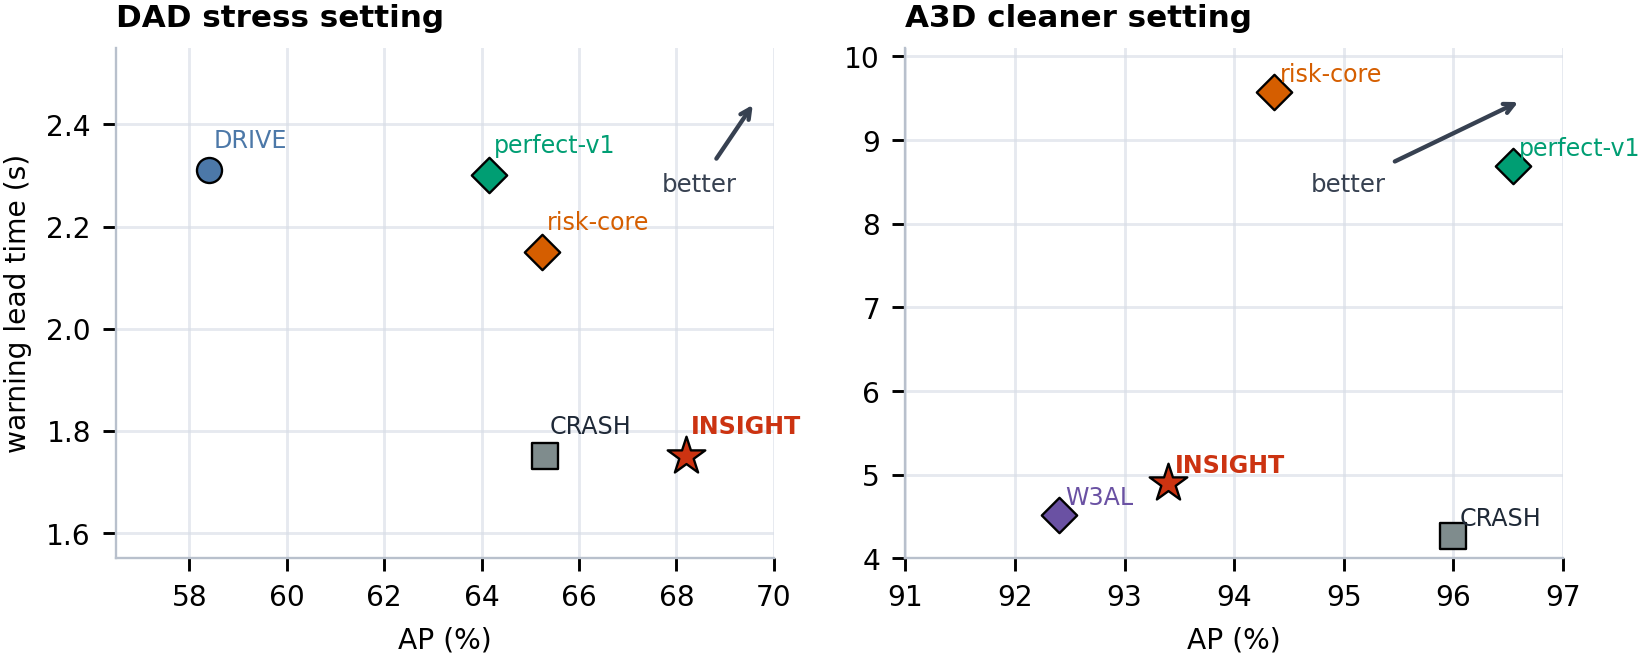
\includegraphics[width=0.98\textwidth]{../figures/emnlp_fig3_operating_points.pdf}
  \caption{\textbf{Safety--utility view.} The same semantic-interface model has
  different readings across datasets: DAD exposes stress and fragility, while
  A3D shows a cleaner AP--warning-time operating point.}
  \label{fig:operating_points}
\end{figure*}

\paragraph{Ontology choice changes the operating point.}
Table~\ref{tab:ontology_polished} is the most direct evidence for the paper's
semantic-interface claim. Only the ontology source changes while the launcher
family is held fixed. On DAD, the compact manual set gives the highest AP while
the polished discovered ontology gives the best mTTA. On A3D, the discovered
ontology has the strongest AP, while the compact manual set gives the best
timing metrics. There is no universally dominant vocabulary; the interface
changes the frontier.

\begin{table*}[t]
\centering\scriptsize
\setlength{\tabcolsep}{2.3pt}
\caption{\textbf{Controlled ontology evidence and scoped diagnostics.}
Ontology cells test the semantic interface directly; support rows explain
mechanism behavior without upgrading stress analyses into headline claims.}
\label{tab:ontology_polished}
\label{tab:concept_sets}
\label{tab:ablation}
\label{tab:trigger_compare}
\label{tab:interp_quant}
\begin{tabular}{p{0.13\textwidth}p{0.18\textwidth}cp{0.08\textwidth}p{0.08\textwidth}p{0.07\textwidth}p{0.28\textwidth}}
\toprule
Block & Condition & \#C & AP$\uparrow$ & mTTA$\uparrow$ & \makecell{TTA@\\R80$\uparrow$} & Reading \\
\midrule
DAD ontology & Historical full & 837 & 64.91\% & 1.88s & 2.51s & Large vocabulary is not automatically better. \\
DAD ontology & Risk-core manual & 30 & \textbf{65.25\%} & 2.15s & \textbf{2.92s} & Compact prior improves DAD AP/timing balance. \\
DAD ontology & Perfect concept set v1 & 80 & 64.15\% & \textbf{2.30s} & 2.67s & Discovered ontology improves lead time. \\
\midrule
A3D ontology & Historical full & 837 & 93.88\% & 9.41s & 8.13s & Strong but broad vocabulary. \\
A3D ontology & Risk-core manual & 30 & 94.36\% & \textbf{9.57s} & \textbf{8.60s} & Best timing under matched launcher. \\
A3D ontology & Perfect concept set v1 & 80 & \textbf{96.54\%} & 8.69s & 7.11s & Best AP in the clean setting. \\
\midrule
Actor source & \makecell[l]{DAD classifier\\$\rightarrow$ actor} & -- & \makecell[l]{61.94\%\\$\rightarrow$34.67\%} & \makecell[l]{2.16s\\$\rightarrow$2.08s} & -- & DAD actor timing remains stress evidence. \\
Actor source & \makecell[l]{A3D classifier\\$\rightarrow$ actor} & -- & \makecell[l]{93.88\%\\$\rightarrow$91.14\%} & \makecell[l]{4.71s\\$\rightarrow$4.97s} & -- & A3D preserves timing behavior better. \\
Intervention & DAD hybrid amplification & -- & -- & -- & -- & Mean alert shift $-2.04$ frames; partial structural intervenability, not causal proof. \\
\bottomrule
\end{tabular}
\end{table*}

\paragraph{DAD robustness and language-side audits.}
Three synchronized DAD curriculum seeds yield 56.39\%$\pm$3.46 AP and
2.40$\pm$0.05s mTTA at epoch 25, and 55.16\%$\pm$3.63 AP and
2.49$\pm$0.09s mTTA at epoch 30. A fixed-vocabulary recovery family improves
the envelope to 63.64\%$\pm$0.80 AP and 2.33$\pm$0.27s mTTA, while a
low-regularization follow-up reaches 64.42\%$\pm$0.97 AP and
2.35$\pm$0.20s mTTA. These runs narrow the gap, but they do not make DAD the
clean mechanism dataset. Language-side audits support the naming policy:
top-3 pseudo-labeling balances coverage and concentration on a 500-frame DAD
slice, and canonical concepts with paraphrases achieve mean text cosine 0.939,
frame-score correlation 0.887, top-10 frame overlap 0.525, and mean absolute
score difference 0.013.

\FloatBarrier
\section{Conclusion}

\method{} reframes accident anticipation around a governed semantic interface.
The central contribution is not a new black-box leaderboard entry, but a method
for building, deploying, and evaluating language-grounded risk concepts as a
trainable model component. Empirically, the interface supports a strong
interpretable operating point, especially on A3D, and controlled ontology
comparisons show that semantic-interface design measurably changes downstream
behavior. The main remaining weakness is DAD-side mechanism fragility and the
gap between classifier-derived anticipation and mature policy-level timing.

\section*{Limitations}
The concept labels are based on CLIP-style pseudo-annotations rather than dense
human frame-level concept supervision. The current ontology is auditable and
reviewed, but not a finished human-validated concept benchmark. The evaluation
uses offline visual features rather than end-to-end video backbones, and
actor-policy timing remains support evidence rather than a complete causal
control account. Deployment would require stronger calibration, robustness, and
human-factors validation.

\bibliography{insight}

\clearpage
\appendix
\section{Extended Analyses, Implementation Details, and Additional Qualitative Results}
\label{sec:appendix}

This appendix expands the main paper in five directions that matter for the
current semantic-interface framing: (i)~implementation detail and reproducibility,
(ii)~additional support for how the semantic interface connects to timing,
(iii)~scoped intervention evidence, (iv)~broader qualitative patterns and
failure cases, and (v)~dataset-specific discussion. The purpose is evidence
traceability: each appendix block makes one part of the semantic-interface
claim easier to inspect, reproduce, or bound.

\paragraph{Reader roadmap.}
Readers mainly interested in reproducibility should start with
Appendix~\ref{app:impl} and Table~\ref{tab:appendix_protocol_trace}. Readers
interested in the language-grounded ontology should continue to
Appendix~\ref{app:concept_pipeline}. Readers concerned about timing and
intervention scope should read Appendix~\ref{app:intervention} together with
the quantitative diagnostics in the main experiments section. Throughout the
appendix, we keep the same boundary as the main paper: \method{} provides a
governed semantic interface with measurable downstream effects, not a finished
policy-level causal benchmark.

\subsection{Implementation Details and Training Protocol}
\label{app:impl}

\paragraph{Input representation.}
Each video is represented as a sequence of per-frame object-centric ROI
features. We use $N{=}19$ object slots per frame and a feature dimension of
$D{=}4096$, following the same object-focused representation used in the main
architecture. For shorter clips, the sequence is padded to the fixed horizon;
for longer clips, we keep the standard anticipation window used by prior work.
This keeps the evaluation protocol aligned with the established accident
anticipation setting rather than introducing a custom temporal crop.

\paragraph{Concept vocabulary.}
The concept bottleneck can be instantiated with either a broad historical
vocabulary or a polished discovered ontology. Our historical setup uses
$K{=}837$ traffic-relevant concepts derived from a large candidate list and
filtered to maintain semantic plausibility for road scenes. The newer concept
pipeline instead constructs a paper-ready ontology through multimodal
large-vocabulary discovery, risk-first refinement, duplicate-cluster
consolidation, family balancing, and very-light human review. The current final
paper-facing discovered ontology contains 80 canonical risk concepts. The
resulting setup therefore gives us two complementary semantic interfaces: a
high-coverage historical vocabulary for legacy comparison and a compact,
auditable, and presentation-ready ontology for concept-set analysis and
next-stage controlled evaluation.

\paragraph{Concept discovery protocol.}
The discovery pipeline begins by sampling pre-crash frames from positive videos
into a frame manifest. A multimodal model is prompted to return candidate risk
concepts, short explanations, and family assignments, with explicit emphasis on
precursor semantics rather than generic scene description. We then apply a
risk-first refinement stage that removes low-value clutter, merges duplicates,
and rewrites phrases into compact risk primitives. Finally, a stronger
adjudicator model canonicalises the surviving concepts, balances semantic
families, and exports a trainable final candidate set. The paper therefore does
not treat the concept vocabulary as a hidden constant: ontology construction is
itself a reproducible algorithmic component.

\paragraph{Prompting and reproducibility.}
The prompt design is deliberately restrictive. We ask for safety-relevant
concepts that can plausibly function as early accident cues, such as closing
distance, cut-in behaviour, lane intrusion, braking onset, occlusion, or
visibility degradation. We discourage static scene trivia, rare one-off object
mentions, and overly dataset-specific wording. In the final paper package we
include prompt templates, JSON schemas, representative raw outputs, and a
controlled ontology-evaluation manifest/launcher so that readers can audit not
only the final ontology but also the intermediate selection process and the
exact evaluation entrypoints used for compact-ontology comparisons.

\paragraph{Pseudo-label binarization.}
For auxiliary concept supervision, we compute cosine similarities between the
CLIP image embedding of frame $t$ and all concept text embeddings. We then set
$\hat{c}_{t,k}=1$ if concept $k$ falls in the frame-wise top-3 similarities and
$\hat{c}_{t,k}=0$ otherwise. This sparse top-$m$ binarization is used in the
main runs reported in the paper; it avoids introducing a global similarity
threshold that would require dataset-specific calibration and keeps the concept
pseudo-targets comparable across ontology sizes. A larger audit over 500
sampled DAD frames from the paper ontology shows why top-3 is a reasonable
compromise: top-1 collapses to only 1.00 concept family per frame on average
and captures 5.5\% of the cumulative top-20 similarity mass, while top-10
expands to 5.14 families per frame and absorbs 51.5\% of that mass. Top-3
yields 2.34 families per frame and 16.0\% relative mass on average, which is
broad enough to avoid extreme concentration but still sparse enough to remain
selective.

\paragraph{Optimisation schedule.}
The total training objective combines classification, concept supervision,
Actor--Critic optimisation, and future-feature distillation. In practice,
these terms do not become useful at the same point in training. The concept
space needs to stabilise before the sequential policy can use it effectively,
and the future-feature distillation term is most helpful when the base visual
representation is already moderately meaningful. For this reason, the training
schedule uses a staged weighting strategy in which the classification and
concept terms dominate early learning, while the sequential decision terms are
allowed to become more influential later. This stabilises optimisation and
empirically avoids the degenerate behaviour where the policy learns to react to
noisy early concepts before those concepts have become semantically coherent.

\paragraph{Hyperparameters.}
In the strongest current configuration, the hidden state size is
$h{=}256$, the concept embedding size is $z{=}128$, the optimiser learning
rate is $2\times10^{-4}$, and the regularisation terms use small but non-zero
weights to avoid overwhelming the main anticipation objective. The concept
alignment, sparsity, and reconstruction losses are all intended as shaping
signals rather than dominant objectives. Their role is to make the bottleneck
more structurally meaningful, not to replace the anticipation loss itself.

\paragraph{Evaluation protocol.}
We report Average Precision (AP), mean Time-To-Accident (mTTA), and the common
threshold-based timing metrics used in prior anticipation work. This is
important because a strong anticipation model must succeed on two axes at once:
it must identify risky videos accurately, and it must do so early enough to be
useful. A method that improves AP while collapsing the warning window is not a
safety win; likewise, a method that warns early at the cost of many false
alarms is not practically deployable. The semantic-interface framing of
\method{} exists partly to address this tension directly.

\paragraph{Rollout and alert rule.}
For a positive video with accident time $\tau$, the agent processes frames in
order and emits either \texttt{wait} or \texttt{alert} at each step. Only the
first alert matters: once emitted, the episode terminates. If no alert is
emitted by frame $\tau$, the episode terminates with a missed-alert penalty.
For a negative video, any alert terminates the episode immediately with a
false-alarm penalty; otherwise the episode ends after frame $T$. In the current
paper, the headline AP/mTTA metrics use the classifier trajectory $p_t$ to
compute the first alert frame, while the actor policy remains an architectural
training component whose large-scale standalone timing reliability is not yet
fully established.

A compact rollout sketch is:
\begin{quote}
\small
for $t=1,\dots,T$: compute $(p_t, \pi_t)$ from $\mathbf{s}_t$;\
if evaluation and $p_t \ge 0.5$: trigger first alert and stop;\
if RL training and $a_t{=}\texttt{alert}$: assign terminal reward and stop;\
if positive clip and $t{=}\tau$ with no alert: assign miss penalty and stop;\
if negative clip and $t{=}T$ with no alert: end episode.\
\normalsize
\end{quote}

\begin{table*}[t]
\caption{Appendix protocol traceability map. This table expands the main-paper
protocol map by tracing each major table or figure to its dataset, ontology,
schedule family, checkpoint rule, seeds, and interpretive role. Its purpose is
to make clear which artifacts support headline prediction, ontology science,
timing support, component isolation, or scoped intervention evidence.}
\label{tab:appendix_protocol_trace}
\centering\scriptsize
\setlength{\tabcolsep}{2pt}
\begin{tabular}{p{0.13\linewidth}p{0.06\linewidth}p{0.10\linewidth}p{0.16\linewidth}p{0.12\linewidth}p{0.05\linewidth}p{0.22\linewidth}}
\toprule
Paper item & Data & Ontology & Schedule family & Checkpoint rule & Seeds & Purpose \\
\midrule
Table~\ref{tab:dad} & DAD & Hist.~837 & Curriculum-stabilized CE+aux+AC+TSD & Canonical single-run line & 1 & Headline interpretable DAD result \\
DAD robustness paragraph & DAD & Hist.~837 & Same clean curriculum family & Fixed epochs 25 and 30 & 3 & Checkpoint-sensitivity diagnostic \\
Table~\ref{tab:a3d} & A3D & Hist.~837 & Shared default CE+aux+AC+TSD & Canonical single-run line & 1 & Headline interpretable A3D result \\
Table~\ref{tab:ablation} & DAD & Hist.~support & Controlled support protocol & Fixed support line & 1 & Component isolation \\
Table~\ref{tab:concept_sets} & DAD/\allowbreak A3D & Hist./risk/\allowbreak perfect & Shared-launcher ontology comparison & One run per ontology-data pair & 1 each & Ontology effect on AP--mTTA trade-off \\
Table~\ref{tab:interp_quant} & DAD & Hist.~archived & Archived timing/intervention analyses & Analysis summaries only & Mixed & Quantitative interpretability diagnostics \\
Figure~\ref{fig:motivation}, Figure~\ref{fig:concept_case_study} & DAD / ontology assets & Mixed & Paper-facing semantic-interface visualization & Curated qualitative selection & -- & Main-paper semantic interface evidence \\
Concept-pipeline figures & Assets & Perfect~v1 & Discovery + consolidation + review pipeline & Asset export & -- & Ontology provenance and auditability \\
Appendix intervention figures & DAD & Hist.~archived & Stored-trajectory + backbone intervention analyses & Archived runnable line & Mixed & Partial intervenability evidence \\
\bottomrule
\end{tabular}
\end{table*}

\begin{table}[t]
\caption{CRS seed audit on the three clean DAD curriculum runs ($7/43/123$). Two seeds retain degenerate all-zero learned risk weights, while one seed learns a non-trivial ranking. The table therefore distinguishes predictive robustness from CRS robustness.}
\label{tab:crs_seed_audit}
\centering\scriptsize
\setlength{\tabcolsep}{3pt}
\begin{tabular}{p{0.14\linewidth}p{0.12\linewidth}p{0.12\linewidth}p{0.12\linewidth}p{0.32\linewidth}}
\toprule
Seed / metric & Epoch & AP$\uparrow$ & mTTA$\uparrow$ & CRS audit \\
\midrule
7 & 20 & 59.97\% & 2.11s & degenerate ($\mathbf{w}_{\text{risk}}\equiv 0$) \\
43 & 15 & 62.33\% & 1.95s & degenerate ($\mathbf{w}_{\text{risk}}\equiv 0$) \\
123 & 110 & 64.62\% & 2.16s & non-trivial ranking learned \\
\midrule
Top-10 overlap & -- & -- & -- & 1.00 for degenerate pair; 0.00 versus informative seed \\
Top-20 overlap & -- & -- & -- & 1.00 for degenerate pair; 0.00 versus informative seed \\
Top-50 overlap & -- & -- & -- & 1.00 for degenerate pair; 0.06 versus informative seed \\
Rank corr. & -- & -- & -- & undefined when one side is degenerate \\
Family consistency & -- & -- & -- & not meaningful without informative rankings in all seeds \\
\bottomrule
\end{tabular}
\end{table}

\begin{figure}[t]
  \centering
  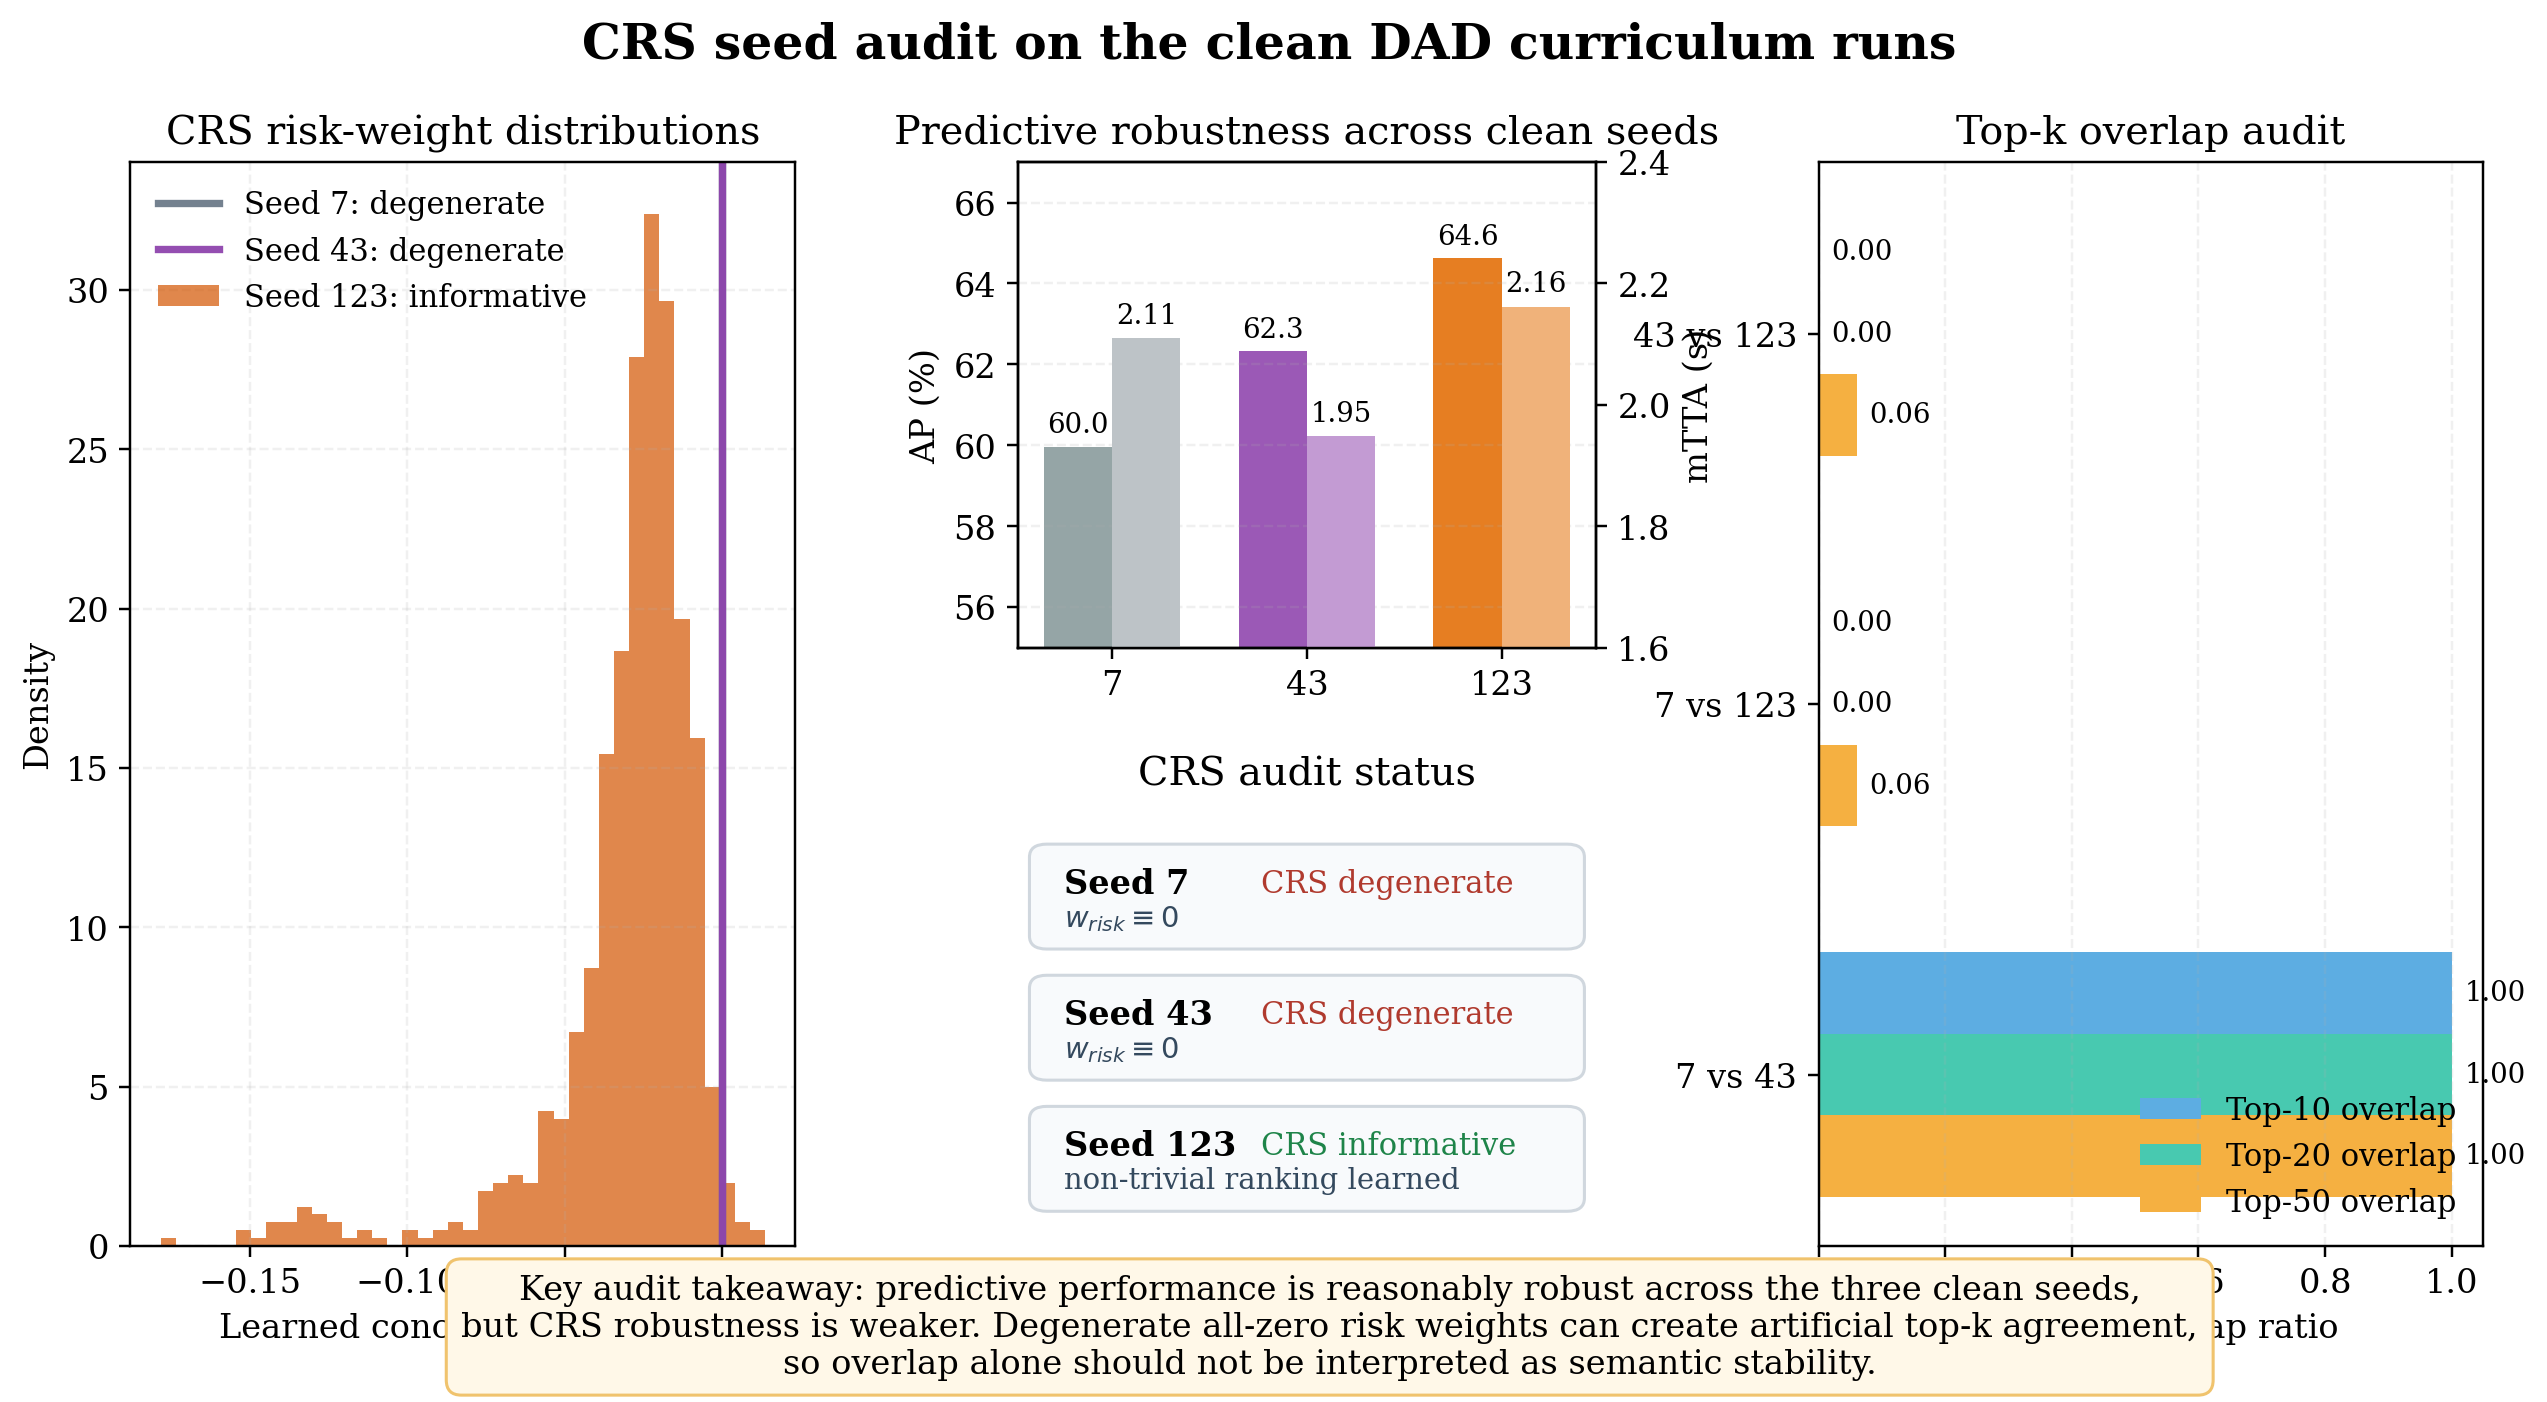
\includegraphics[width=0.98\linewidth]{../figures/insight_fig_appendix_crs_seed_audit.pdf}
  \caption{\textbf{CRS seed audit on the clean DAD curriculum runs.}
  Left: the learned CRS risk-weight distribution is degenerate for seeds 7 and
  43 (all-zero weights), while seed 123 learns a non-trivial ranking.
  Middle: predictive metrics remain reasonably similar across seeds, showing
  that predictive robustness and CRS robustness are not the same phenomenon.
  Right: pairwise top-$k$ overlap is high only for the degenerate pair and
  collapses against the informative seed, so overlap alone should not be read
  as evidence of semantic stability.}
  \label{fig:appendix_crs_seed_audit}
\end{figure}

\paragraph{Why this CRS audit matters.}
Reviewer-facing stability claims should distinguish \emph{predictive robustness}
from \emph{CRS robustness}. The three clean DAD seeds remain useful for the
former, but Table~\ref{tab:crs_seed_audit} and
Figure~\ref{fig:appendix_crs_seed_audit} show that they do not yet support a
strong claim that the learned concept-risk ranking is stable across seeds.
In particular, two of the three clean seeds are degenerate, while only one
learns a non-trivial CRS ranking. This means the current clean-seed degeneracy
rate is $2/3$, and it also means that top-$k$ overlap and family-level
agreement are not genuinely informative stability statistics at present because
there is only one informative seed in the audited pool. This motivates the
paper's current cautious wording: the semantic interface is architecturally
meaningful and partially supported quantitatively, but CRS should currently be
understood as a \emph{tentative audit signal} rather than as a mature,
deployment-ready inspector interface. A stronger multi-seed CRS stability study
should therefore be viewed as an explicit next validation target rather than as
a completed result.

\paragraph{Trigger-source support beyond one checkpoint.}
We also extended the actor-versus-classifier comparison beyond the single
representative DAD checkpoint used in the main table. Across six same-family
curriculum checkpoints, classifier-based trigger evaluation averages
$61.11\%\pm4.58$ AP and $2.17\pm0.19$~s mTTA, while actor-based trigger
evaluation averages $37.41\%\pm7.35$ AP and $3.73\pm1.39$~s mTTA. The mean
actor threshold-crossing rate at $0.5$ is only $0.68\pm0.43$, which exposes a
second source of instability: even when the actor emits usable timing behavior
on some checkpoints, its crossing dynamics are not yet consistent enough to
serve as the main paper metric path.

\subsection{Concept Ontology Construction: Additional Details}
\label{app:concept_pipeline}

\paragraph{Why this appendix section matters.}
A natural concern is whether our concepts are merely a fixed word list
chosen by hand. The answer is no. The current project contains a full pipeline
for constructing and comparing accident-risk ontologies, and this appendix
makes that process explicit so that the semantic interface of \method{} can be
audited as carefully as the neural architecture itself.

\paragraph{Ontology evolution across stages.}
Table~\ref{tab:concept_evolution} summarises the ontology evolution that is
actually relevant for the current paper. The progression is now sharper than in
earlier drafts: we begin with a broad historical vocabulary for high-coverage
training, keep a compact manual risk-core set as a human-prior baseline, and
then construct a paper-ready discovered ontology through large-vocabulary
mining, risk-first consolidation, family balancing, naming normalization, and
very-light human review. Figure~\ref{fig:concept_evolution} complements the
table with representative examples from these stages, while
Figure~\ref{fig:concept_case_study} makes the merge provenance concrete through
real canonicalization examples.

\begin{figure*}[t]
  \centering
  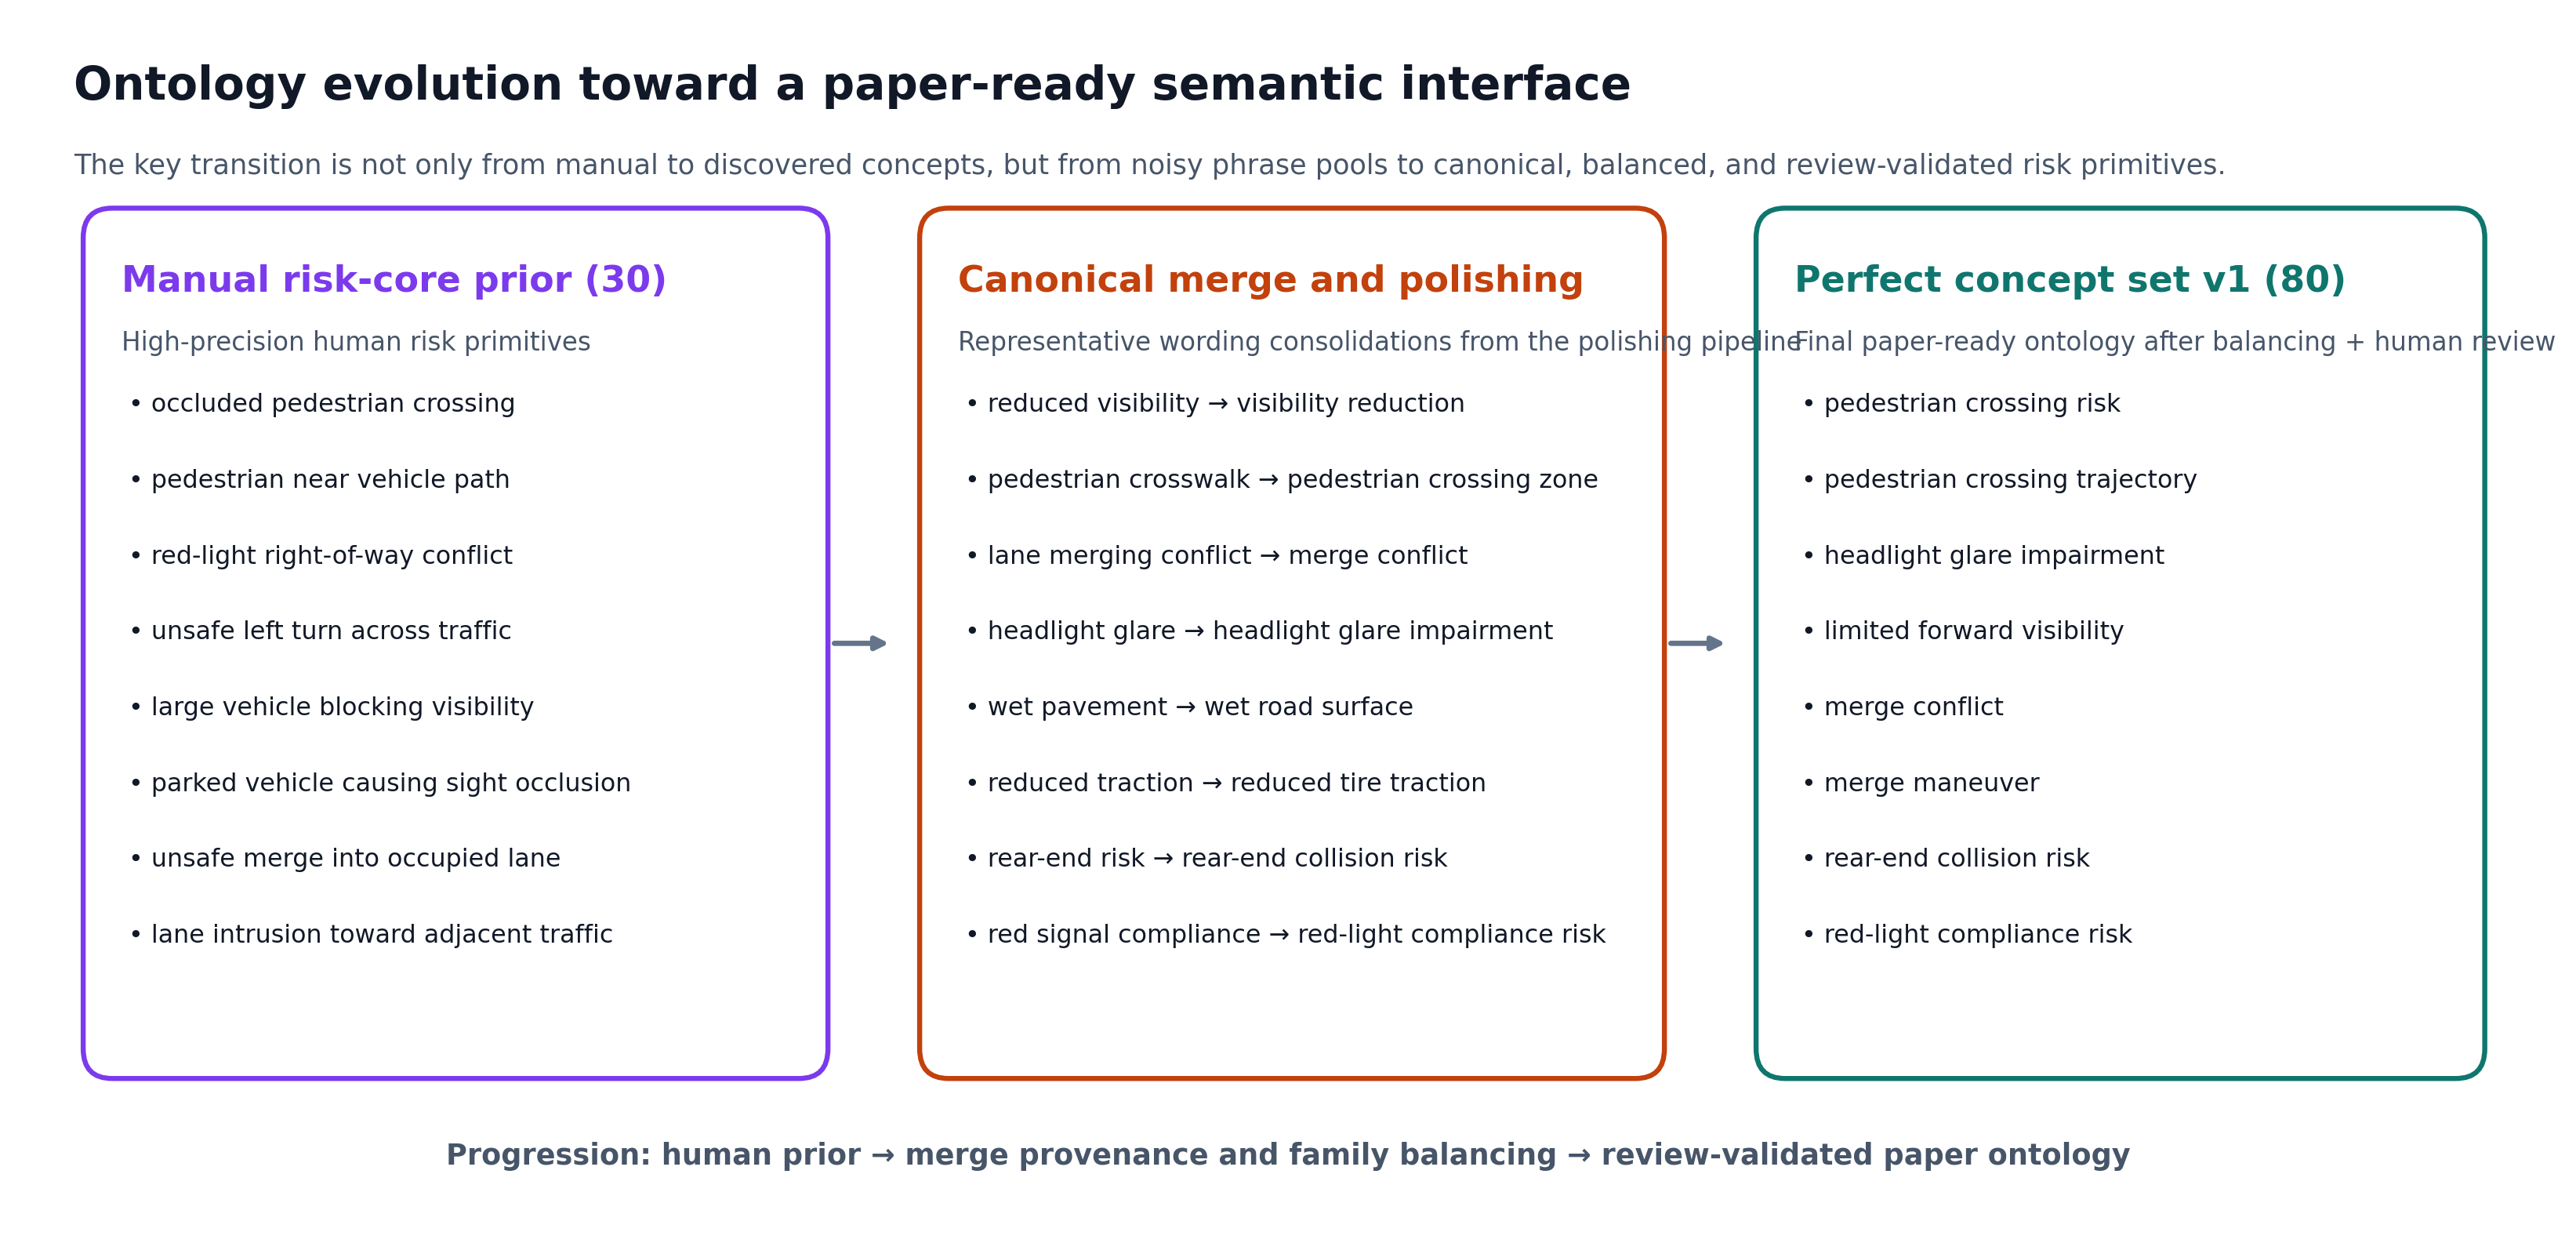
\includegraphics[width=0.98\textwidth]{../figures/insight_fig_concept_evolution.pdf}
  \caption{\textbf{Ontology evolution toward a paper-ready semantic interface.}
  Left: the manual risk-core ontology encodes strong human priors about accident
  precursors. Middle: representative merge and canonicalization examples from
  the polishing pipeline show how noisy or fragmented phrase clusters are
  compressed into stable risk primitives. Right: the final \emph{Perfect concept
  set v1} provides a balanced and review-validated ontology that is both more
  readable than the broad historical pool and more mature than early compact
  discovered pilots.}
  \label{fig:concept_evolution}
\end{figure*}

\begin{table}[t]
\caption{Concept ontology evolution across the project.}
\label{tab:concept_evolution}
\centering\small
\setlength{\tabcolsep}{4pt}
\resizebox{\linewidth}{!}{%
\begin{tabular}{lccp{0.42\linewidth}}
\toprule
Stage & \#Concepts & Source & Main property \\
\midrule
Historical full vocabulary & 837 & Broad CLIP-derived concept bank & High coverage, historically strongest CBM line, but semantically noisy and too large for clean paper presentation \\
Risk-core manual set & 30 & Manual risk-first curation & High-precision compact human prior over accident precursors \\
Perfect concept set v1 & 80 & Large-vocab discovery + polishing + human review & Balanced paper-ready ontology with canonical naming, merge provenance, explicit family coverage, and exhaustive per-concept review \\
\bottomrule
\end{tabular}%
}
\end{table}

\paragraph{Controlled ontology block status.}
The shared-launcher ontology comparison described in the main paper is now
complete as an artifact block: all six recommended runs
(\texttt{DAD/A3D} crossed with \texttt{historical\_full},
\texttt{risk\_core\_v1}, and \texttt{perfect\_v1}) are present with stored
checkpoints and \texttt{results.json} summaries. This matters because the
ontology claim is no longer resting on planned compute. On DAD, the compact
manual ontology achieves the highest AP while the polished discovered ontology
achieves the best mTTA; on A3D, the polished ontology achieves the strongest AP
while the compact manual ontology gives the best timing metrics. In other
words, the appendix now supports the main-paper reading directly: ontology
choice changes the operating point under one matched recipe.

The seed-backed extension of this block is also complete: all $18/18$
recommended seeded ontology runs have finished. This matters because the
ontology claim no longer depends on a half-completed follow-up.
The aggregate picture is consistent with the main paper's interpretation. On
A3D, the polished discovered ontology remains a strong AP-oriented operating
point under three seeds ($93.35\%\pm0.49$ AP), while on DAD the same ontology
is visibly more variable ($60.11\%\pm7.40$ AP). We therefore read the multi-seed
results as strengthening the ontology-science claim while also sharpening the
paper's limitation statement: the semantic interface looks materially more
stable on A3D than on DAD.

\paragraph{Prompt template design.}
Our prompts explicitly instruct the multimodal model to prioritise
\emph{safety-relevant early cues} rather than generic scene description.
Representative output fields include a compact concept phrase, a short risk
rationale, and a semantic family tag. A simplified prompt sketch is:
\begin{quote}
``Given a pre-crash driving frame, list short risk concepts that could function
as accident precursors. Prefer dynamic hazard cues, proximity conflict,
visibility degradation, braking or cut-in behaviour, and lane-level conflict.
Avoid generic objects or background scene tags unless they directly contribute
to accident risk.''
\end{quote}
We pair this instruction with a structured JSON schema so that outputs can be
programmatically filtered, clustered, and adjudicated. A representative schema
fragment is shown below.

\begin{quote}
\small
\noindent\parbox{0.95\linewidth}{\raggedright\ttfamily
\{"frame\_id": "dad\_xxx\_f042",\\
"risk\_concepts": [\\
\hspace*{1em}\{"concept": "trajectory conflict",\\
\hspace*{2em}"family": "motion\_conflict",\\
\hspace*{2em}"why\_risky": "vehicles are converging into\\
\hspace*{2em}the same path"\},\\
\hspace*{1em}\{"concept": "forward visibility limit",\\
\hspace*{2em}"family": "visibility",\\
\hspace*{2em}"why\_risky": "driver cannot reliably\\
\hspace*{2em}anticipate hidden hazards"\}\\
],\\
"discarded\_scene\_tags": ["road", "car", "intersection"]\\
\}}
\normalsize
\end{quote}

\paragraph{Concrete examples from the current polishing pipeline.}
The manual risk-core set contains phrases such as \emph{lane intrusion toward
adjacent traffic}, \emph{oncoming-traffic conflict}, and \emph{large vehicle
blocking visibility}. The newer large-vocabulary discovery stage produces a
much broader phrase pool that includes many useful but fragmented variants,
such as \emph{reduced visibility}, \emph{pedestrian crosswalk},
\emph{lane merging conflict}, or \emph{wet pavement}. The polishing stage then
consolidates these into canonical training-ready forms such as
\emph{visibility reduction}, \emph{pedestrian crossing zone},
\emph{merge conflict}, and \emph{wet road surface}. Including both raw and
canonical forms is important: it shows how the pipeline moves from high-recall
multimodal phrase mining toward a smaller, more stable, and more reviewable
ontology without losing the underlying risk semantics.

\paragraph{Failure modes in raw discovery.}
The raw discovery stage is intentionally high recall and therefore noisy.
Typical failure modes include: (i) generic object mentions that carry little
predictive value (e.g., ``road'', ``vehicle''), (ii) visually salient but weakly
risk-relevant background phrases, (iii) duplicate concepts with slightly different
wording, and (iv) over-specific phrases that do not transfer across clips.
These failure modes are precisely why the refinement and adjudication stages
are necessary; they are not implementation accidents, but expected properties
of an intentionally recall-heavy front end.

\paragraph{Why polishing plus human review is useful.}
The final ontology stage does more than clean spelling. It rebalances semantic
families, collapses near-synonyms, enforces canonical naming, and applies a
very-light human review over every retained concept. This matters for both
science and engineering: the method needs a reproducible ontology with visible
provenance, and the downstream model wants a small set of stable concepts
rather than a fragile bag of aliases. Figure~\ref{fig:concept_case_study} shows
representative real merge examples from this process, moving from noisy raw
multimodal phrases to final canonical concepts that can be presented in the
paper and used directly for downstream CBM training.

The current audit trail makes this concrete. Starting from 611 mined phrases,
the polishing pipeline compresses the pool to 81 post-polish canonical
candidates and a finalized paper release of 80 retained concepts. The review
record spans all 80 retained concepts across nine semantic families, and the
documented decisions are intentionally light-touch: wording is checked and
canonicalized, but the ontology is not rebuilt by hand. This is the level of
governance we want the paper to claim: explicit canonical naming, visible merge
provenance, and family balance that can be inspected by a reader without
pretending that the vocabulary is a finished standalone linguistic resource.

\paragraph{What the language-side evidence is meant to establish.}
The paper does not claim that these canonical names are universally optimal or
that the ontology has become a finished linguistic resource. The narrower and
more defensible claim is that the ontology is governed enough to function as a
scientific interface: canonical names remain reasonably stable under light
paraphrase variation, semantic families are explicit rather than implicit, and
merge choices are reviewable rather than hidden inside prompt iteration.

\begin{figure*}[t]
  \centering
  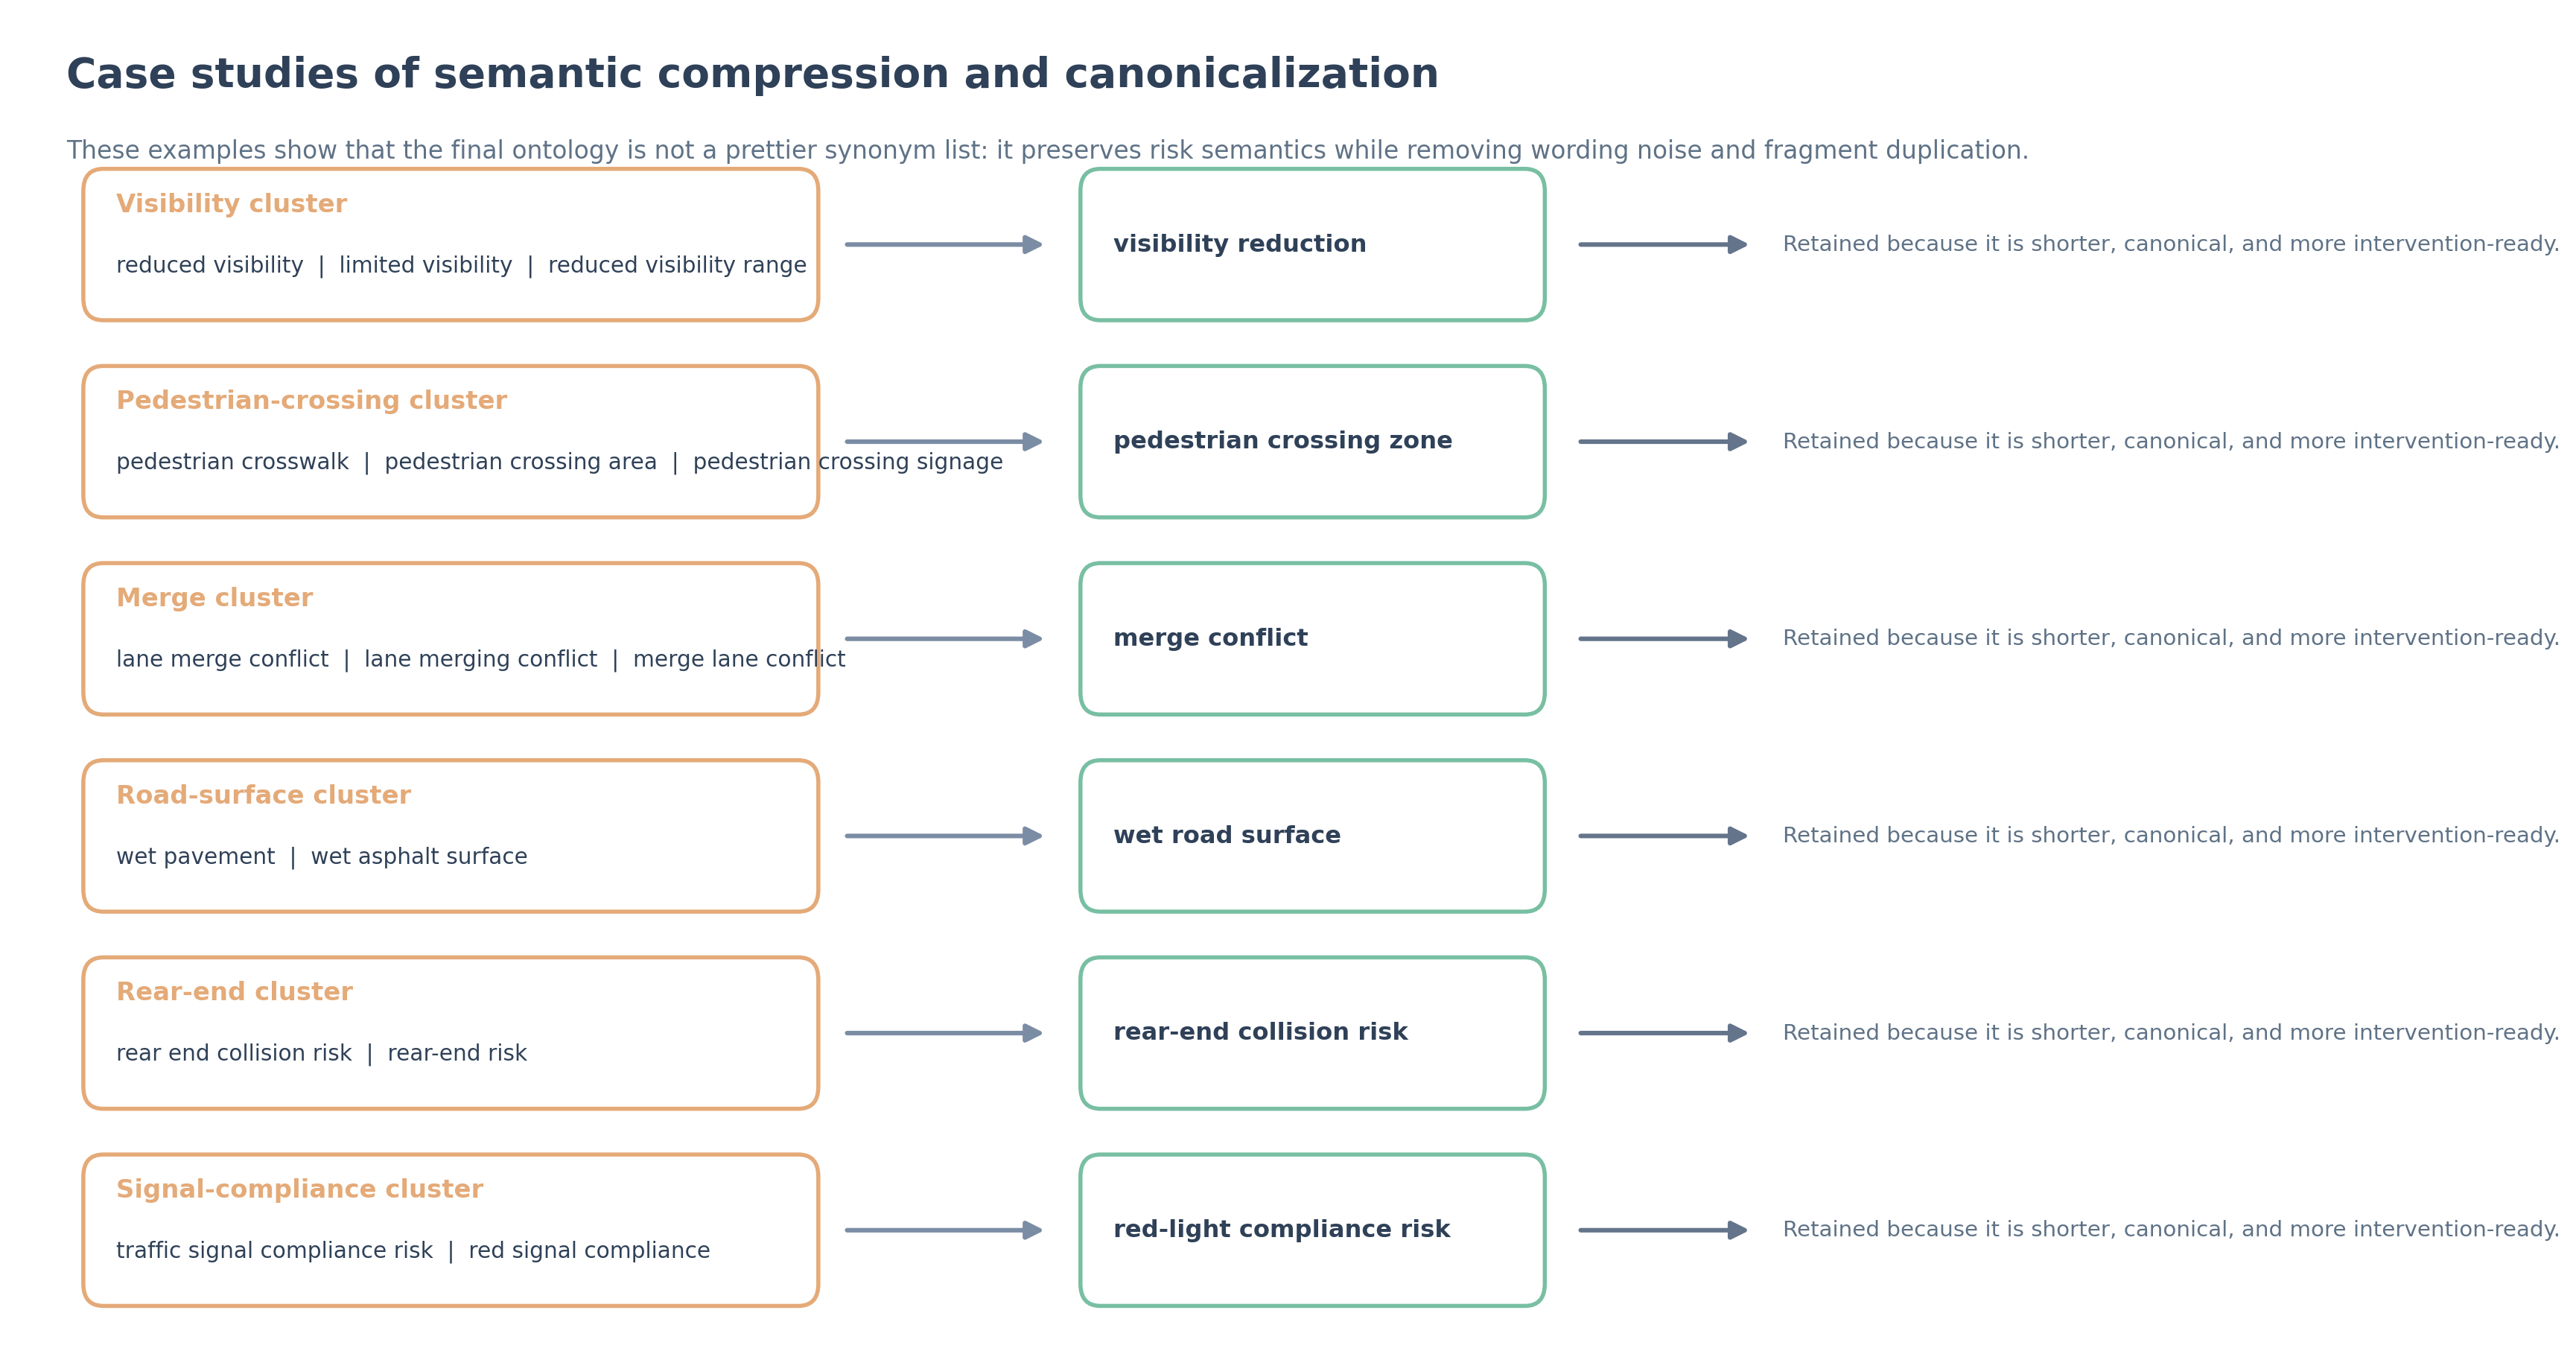
\includegraphics[width=0.98\textwidth]{../figures/insight_fig_concept_case_study.pdf}
  \caption{\textbf{Case studies of semantic compression and canonicalization.}
  Each row shows a representative merge path from noisy or fragmented phrase
  variants to a single canonical paper-ready concept. These examples make two
  points explicit: the pipeline removes lexical fragmentation, and the final
  ontology is not merely a prettier synonym list but a more stable semantic
  interface for downstream CBM training, family-level analysis, and external
  auditing.}
  \label{fig:concept_case_study}
\end{figure*}

\paragraph{What counts as success.}
A discovered concept set is successful only if it satisfies four criteria:
(1) semantic plausibility to a human reader, (2) coverage of major accident
precursor families, (3) trainability in the downstream CBM pipeline, and
(4) auditability at the paper level through family metadata, merge provenance,
and human review. This is why the paper reports not only ontology examples and
downstream training results, but also family-balance figures and merge case
studies. A pretty concept list without learning value is not enough; conversely,
a trainable but uninterpretable list would defeat the purpose of the semantic
interface.

\begin{figure}[t]
  \centering
  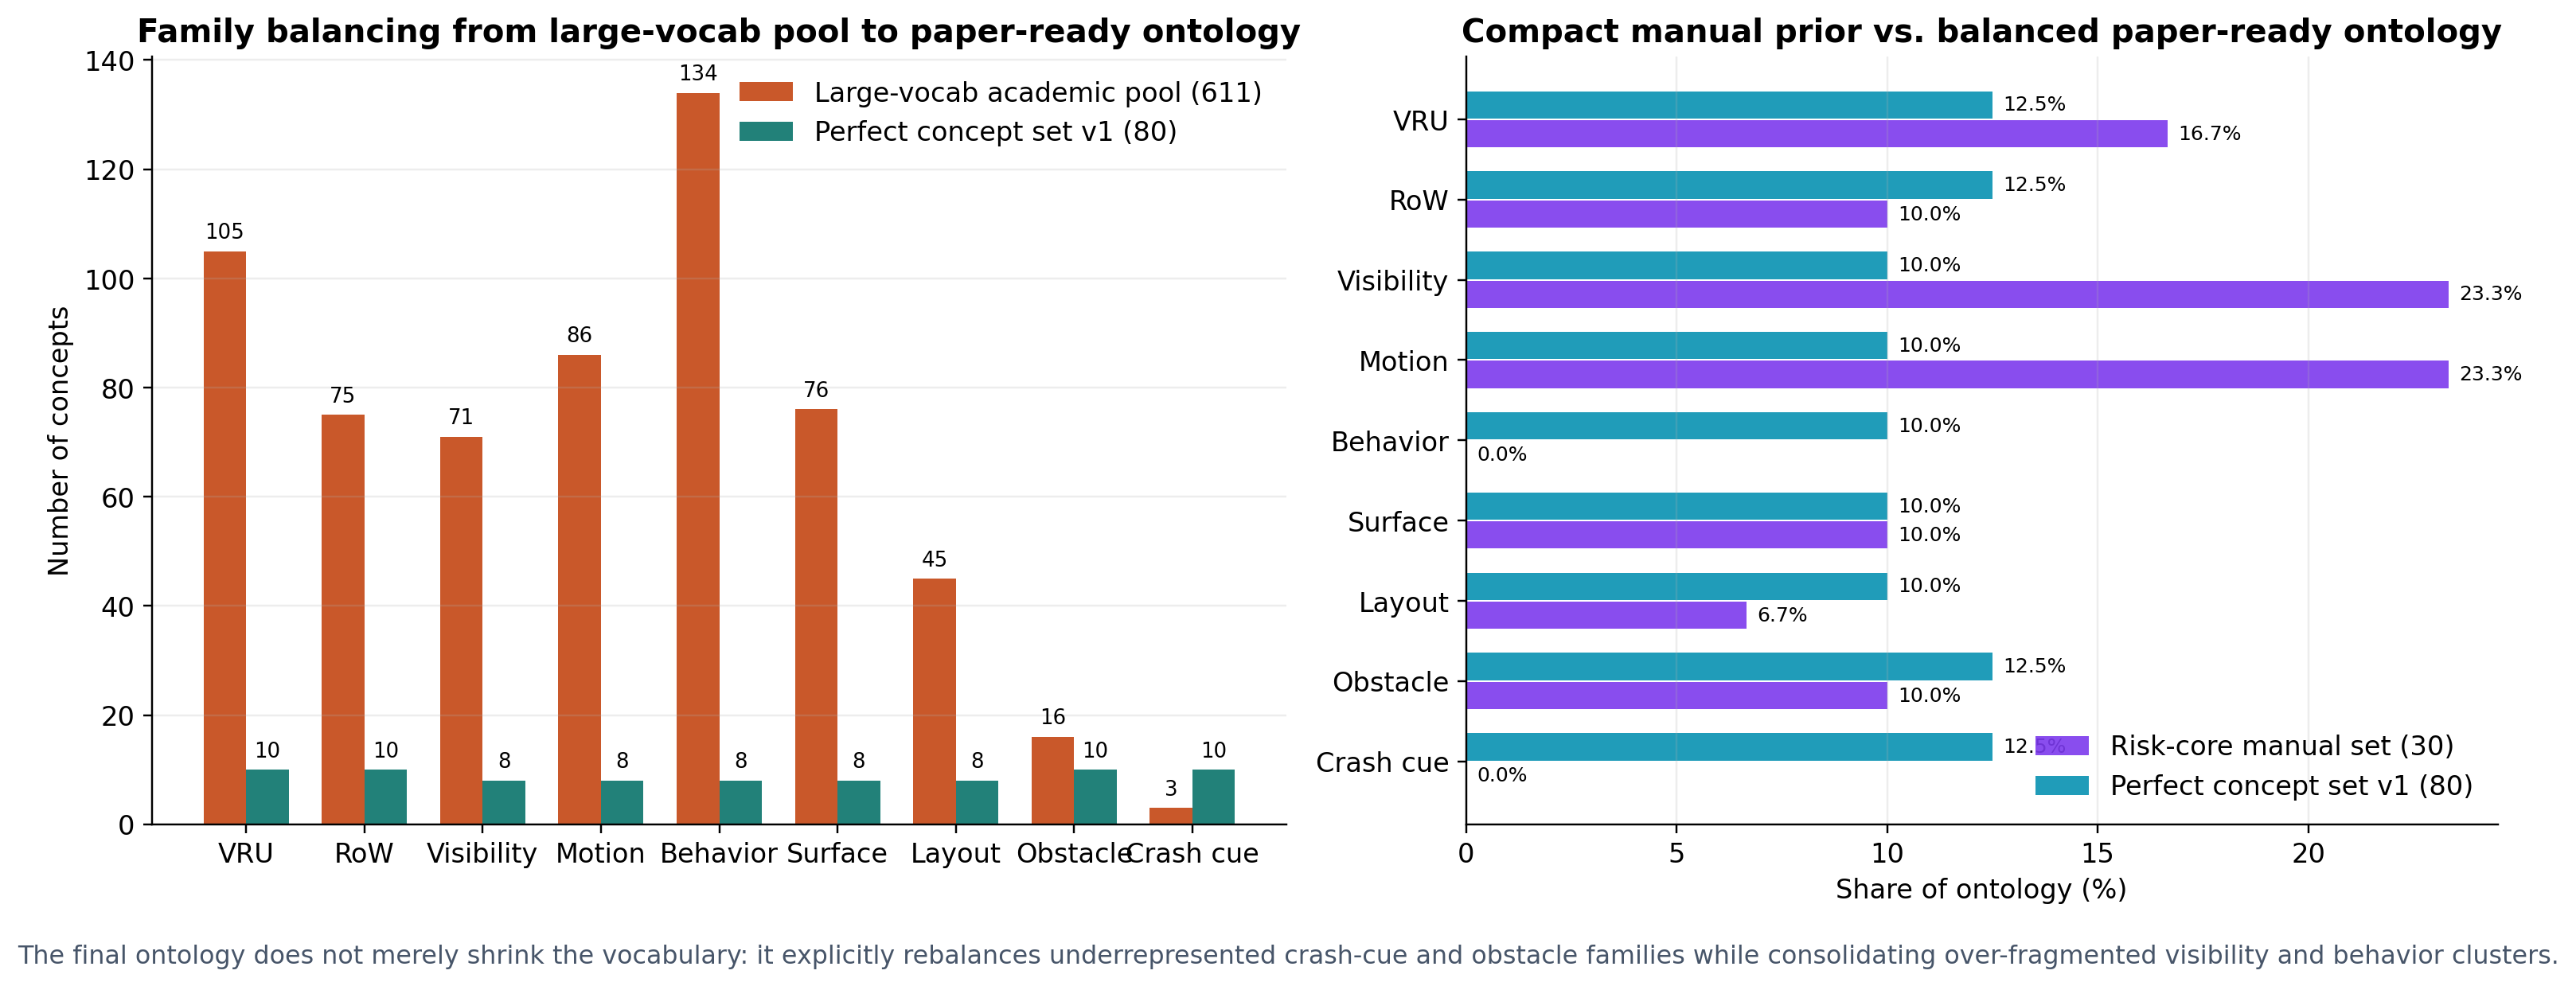
\includegraphics[width=0.98\linewidth]{../figures/insight_fig_concept_family_coverage.pdf}
  \caption{\textbf{Family coverage before and after ontology polishing.}
  The broad large-vocabulary pool is highly imbalanced, while the final paper-ready
  ontology explicitly rebalances crash-cue, obstacle, and vulnerable-road-user
  families without collapsing the ontology into a tiny manually curated list.
  This supports our claim that ontology polishing is not cosmetic compression;
  it is a structured operation that improves auditability and semantic balance.}
  \label{fig:concept_family_coverage}
\end{figure}

\subsection{Why the Semantic Interface Can Affect Timing}
\label{app:theory}

\paragraph{From latent prediction to semantic decision-making.}
A conventional recurrent anticipation model compresses all evidence into a
single latent state $\mathbf{h}_t$ and predicts risk from that state alone.
This is often sufficient for raw prediction, but it is weak from an auditing
perspective because the model offers no explicit separation between
\emph{evidence extraction} and \emph{decision timing}. By contrast, \method{}
explicitly decomposes these two roles:
\begin{itemize}[leftmargin=1.5em]
  \item the \textbf{semantic layer} estimates a concept state $\mathbf{c}_t$ that
  summarises semantically meaningful risk evidence, and
  \item the \textbf{timing layer} learns a timing policy over a concept-aware
  sequential state $\mathbf{s}_t=[\mathbf{h}_t\|\mathbf{c}_t]$.
\end{itemize}
This decomposition is not cosmetic. It changes the information geometry of the
problem: the policy no longer acts on an opaque hidden vector alone, but on a
state with an explicit semantic interface.

\paragraph{A simple monotonicity view.}
Suppose the concept state contains one or more dimensions corresponding to
hazard indicators whose increase is semantically consistent with increasing
risk. If the downstream timing policy is trained to reward earlier correct
alerts, then a policy conditioned on $\mathbf{s}_t=[\mathbf{h}_t\|\mathbf{c}_t]$
can, in principle, cross the alert boundary before a purely confidence-based
predictor reaches its peak. Informally, the concept channel acts as an early
warning basis: a rise in concept evidence can move the system toward action
before the latent classifier has accumulated maximal confidence. This is the
core reason the semantic and timing layers are coupled but not redundant.

\paragraph{Why intervention is meaningful.}
Let a concept edit be represented as a perturbation
$\Delta\mathbf{c}_t$ applied over a short pre-crash window.
Because the downstream predictor or policy consumes a state containing the
concept vector, the perturbation induces a corresponding perturbation in the
decision state:
\[
\mathbf{s}'_t = [\mathbf{h}_t\|\mathbf{c}_t + \Delta\mathbf{c}_t].
\]
If the architecture is truly concept-conditioned rather than merely
post-hoc-explainable, then semantically valid positive perturbations on a risk
concept should induce a stronger or earlier warning response at the output.
This is why the intervention analysis is an architectural test, not just a
visualisation trick. The test asks whether the semantic interface has
non-trivial structured influence on the decision pathway.

\paragraph{What this appendix-level analysis does and does not claim.}
We do not claim a formal global theorem guaranteeing monotone policy shifts for
all concept edits, since the recurrent dynamics and nonlinearities are too rich
for such a guarantee to be informative without unrealistic assumptions. The
point of the analysis is instead to make clear why the design is principled:
separating semantic evidence estimation from timing control creates a decision
pathway that is inspectable, perturbable, and therefore much closer to the
needs of safety auditing than a single black-box recurrent score.

\subsection{Scoped Intervention Evidence}
\label{app:intervention}

A standard promise of concept bottleneck models is \emph{intervenability}: a
human can inspect a concept, judge that it is mis-estimated, and correct it
without retraining the full network. For accident anticipation, this capability
is especially important because many practically relevant errors are not
arbitrary; they are tied to under-activation of an intuitively correct risk
concept. In the current paper, however, intervention should be read as
\emph{support evidence} for a meaningful semantic control surface, not as a
completed policy-level causal benchmark.

\begin{figure*}[t]
  \centering
  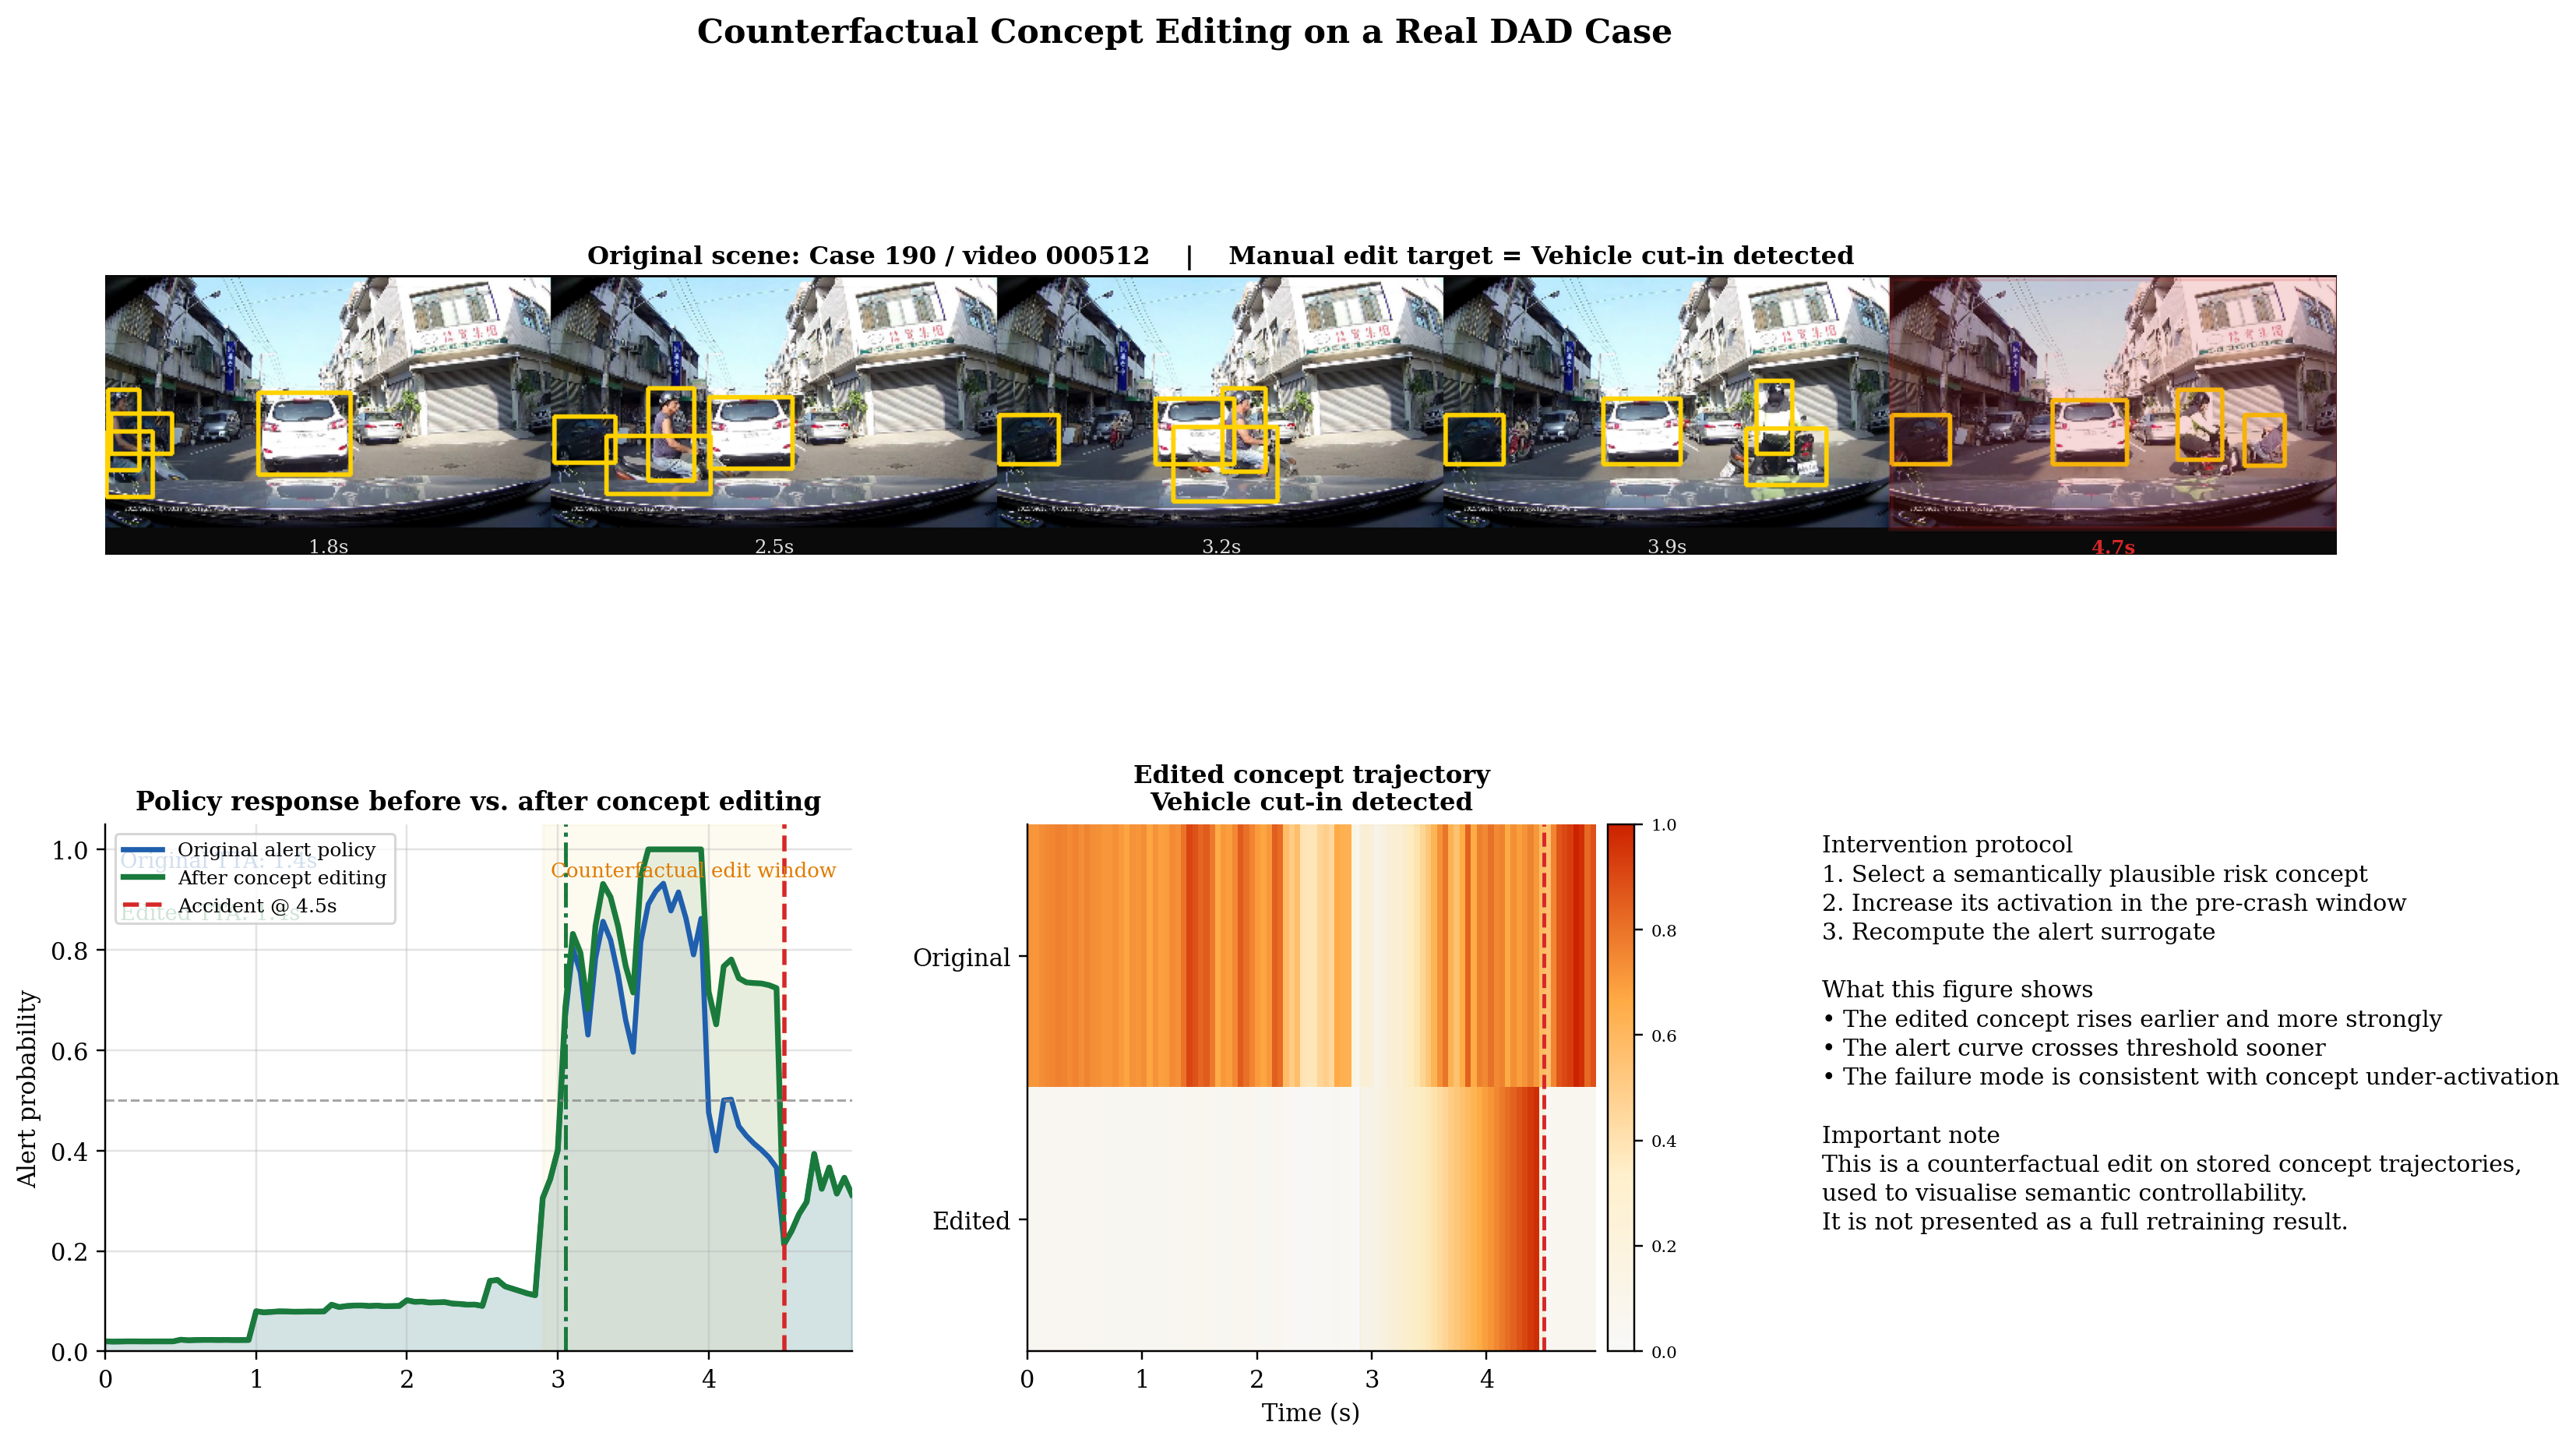
\includegraphics[width=\textwidth]{../figures/insight_fig_appendix_intervention.pdf}
  \caption{\textbf{Counterfactual concept editing on a DAD case.}
A semantically plausible pre-crash concept trajectory is increased and the
resulting warning surrogate is recomputed. The edited concept rises earlier,
and the alert curve crosses threshold sooner. This figure is intentionally a
stored-trajectory counterfactual rather than a full model re-run; its role is
to show that the model exposes a semantically meaningful control surface.}
  \label{fig:appendix_intervention}
\end{figure*}

\paragraph{Stored-trajectory intervention protocol.}
For a false-negative or borderline DAD case, we select a concept whose
activation is visibly inconsistent with the scene semantics, increase it over
the pre-crash window, and compare the original and edited warning trajectories.
This directly tests whether strengthening the right concept can move the
warning earlier.

\paragraph{Outcome.}
Figure~\ref{fig:appendix_intervention} shows that it can. The edited alert
curve rises and crosses threshold earlier than the original one. Across the
archived quantitative summaries, however, the effect remains heterogeneous. In
the strongest archived hybrid-boost setting, the mean alert shift is
$-2.04$ frames over 64 cases, but the median shift is still 0.0; by contrast,
both the null-style hybrid baseline and the risk-weight baseline produce a mean
shift of 0.0 over 32 cases each. The correct interpretation is therefore
\emph{partial structural intervenability} rather than a completed causal proof.

\begin{figure*}[t]
  \centering
  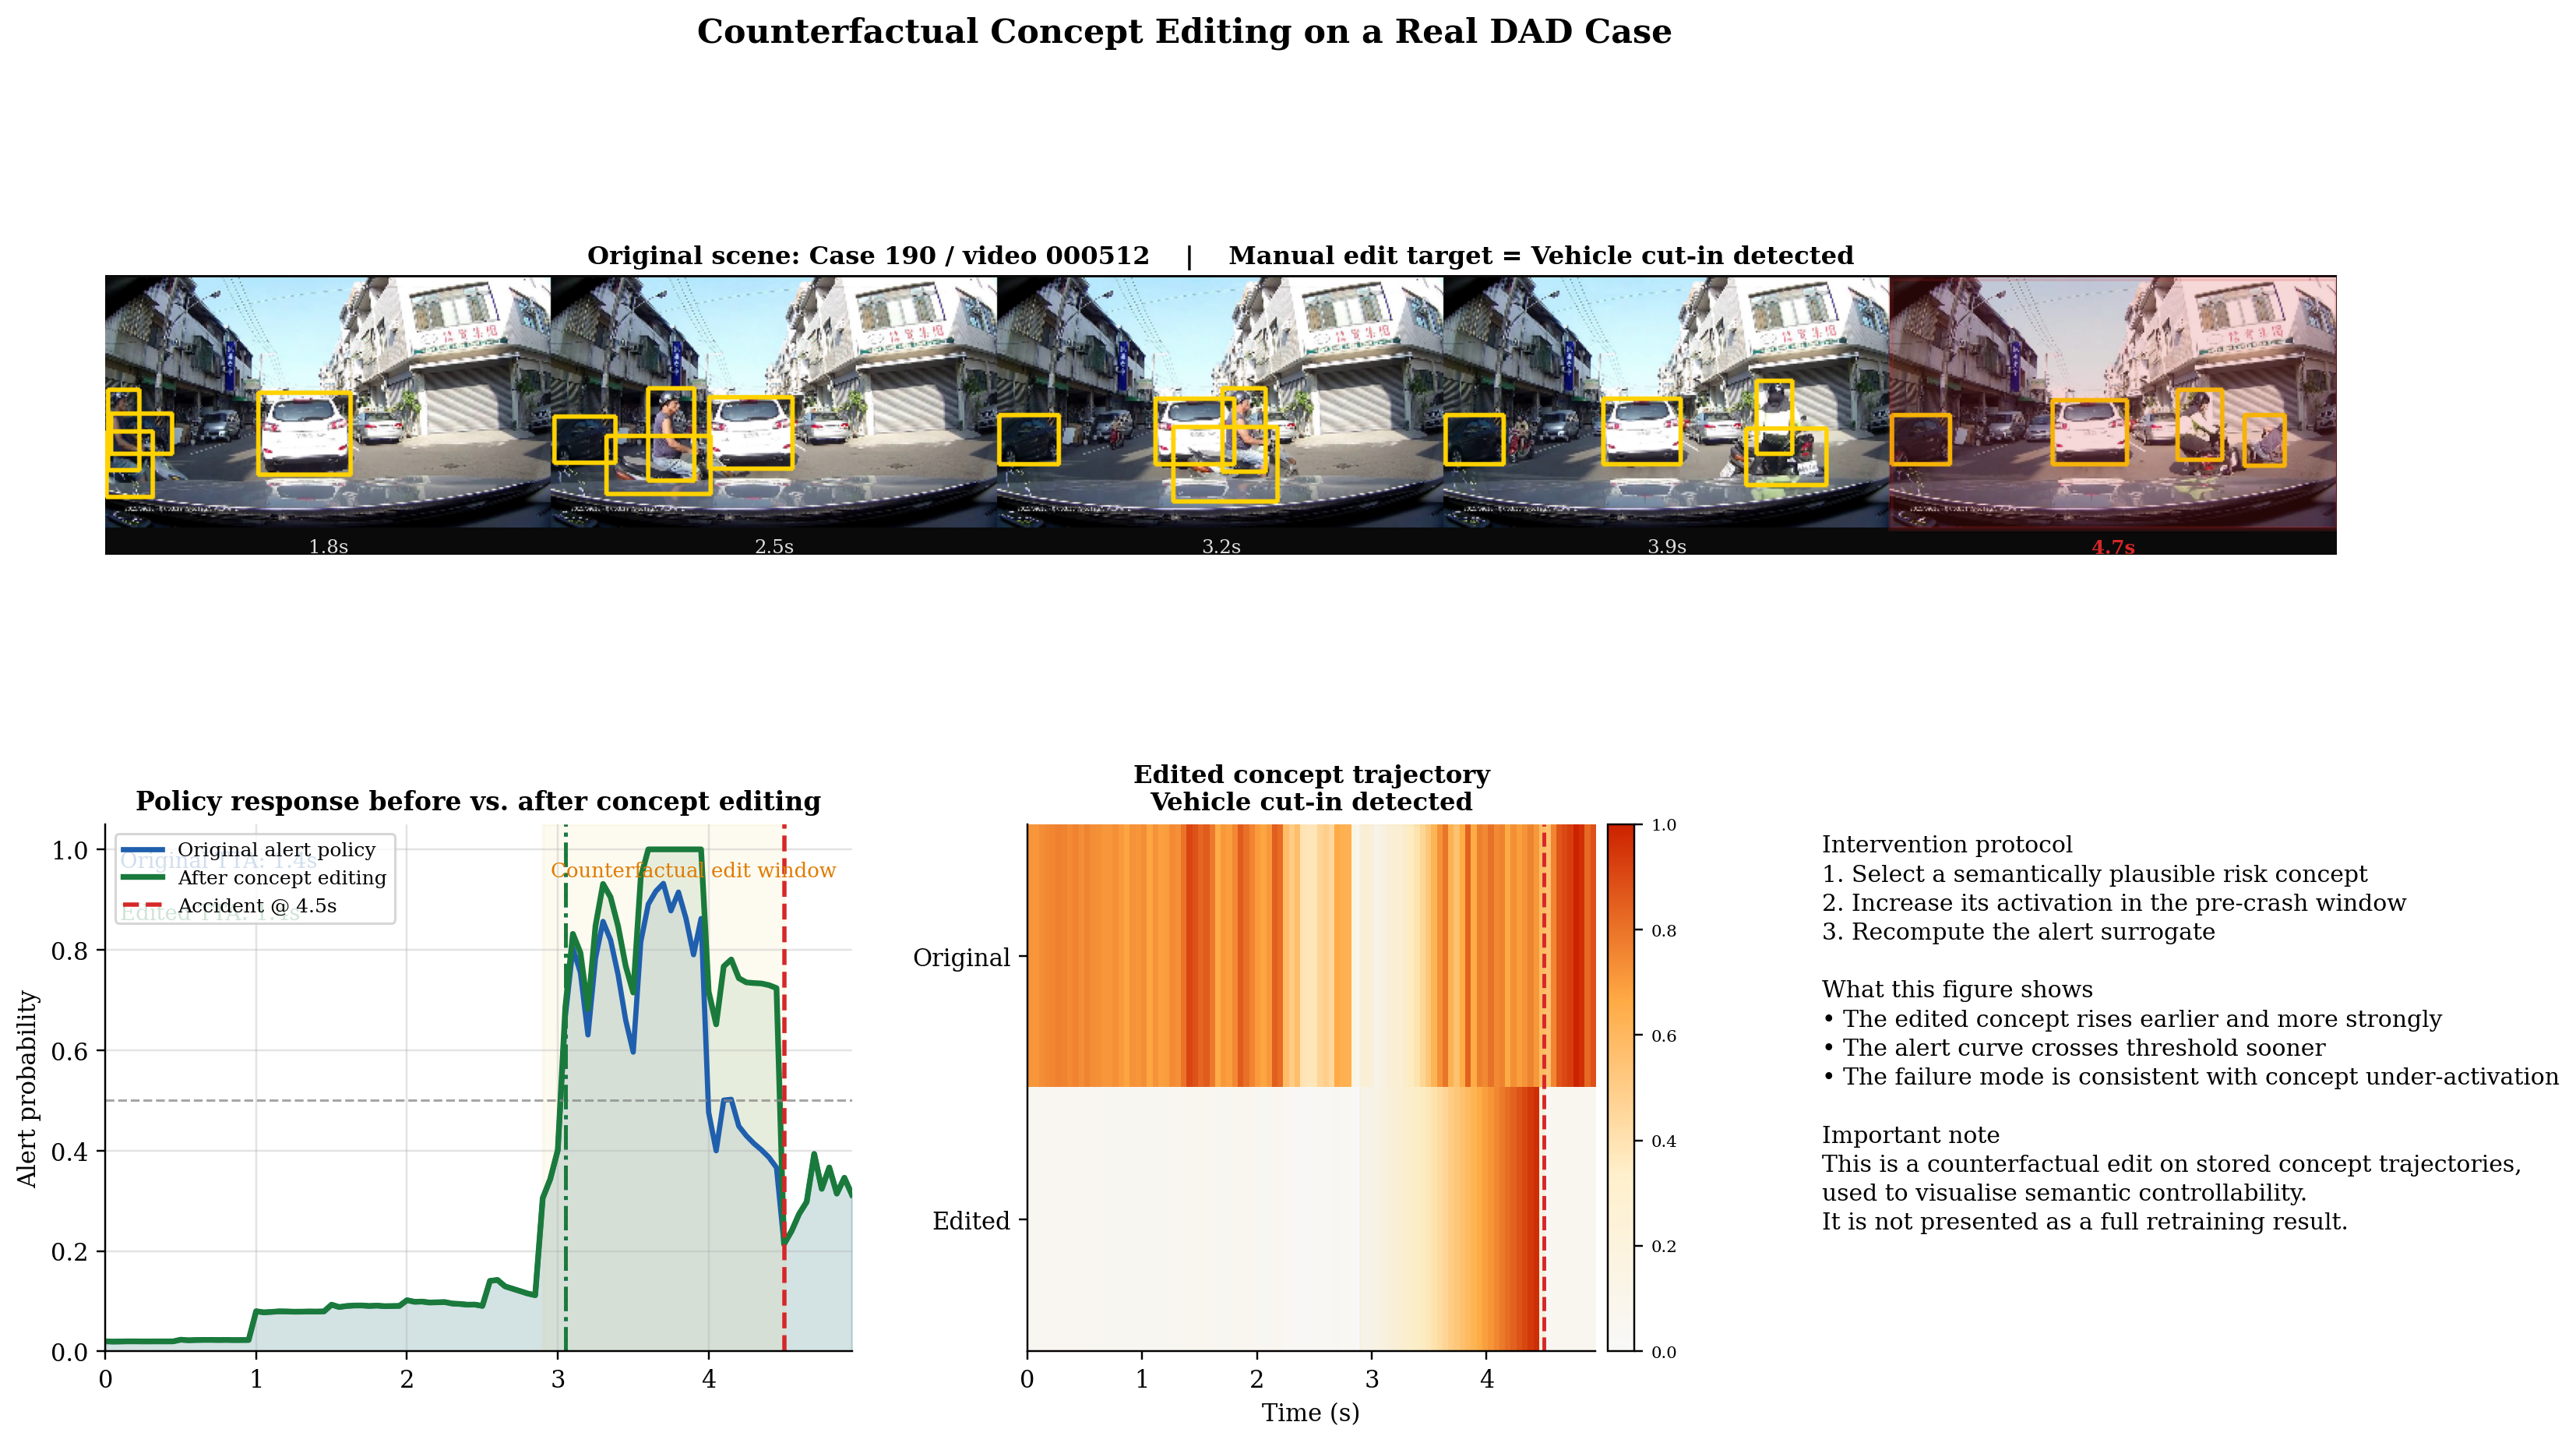
\includegraphics[width=\textwidth]{../figures/insight_fig_appendix_intervention_v4_backbone.pdf}
  \caption{\textbf{Backbone-level intervention re-run with the v4 DAD checkpoint.}
A concept channel is edited in the pre-crash window and the downstream
prediction branch is recomputed through the loaded backbone. This is a stronger
intervention path than stored-trajectory editing, but it is still not a full
policy-level intervention because the available checkpoint lacks the final
Actor--Critic head weights.}
  \label{fig:appendix_intervention_v4}
\end{figure*}

\paragraph{Backbone-level re-run.}
To go beyond stored-trajectory editing, we also run a backbone-level
intervention using the newer DAD line. The available checkpoint loads the
concept bottleneck, temporal modules, and recurrent backbone, but not the final
Actor--Critic head weights. We therefore edit one concept channel and recompute
the downstream prediction branch through the loaded backbone.

\paragraph{Interpretation.}
The backbone-level re-run shows that concept edits remain meaningful when
propagated back through the loaded model rather than only visualised post hoc.
It also makes the current evidence boundary explicit: we can support a
concept-conditioned backbone intervention, but not yet a full policy-level
intervention without the complete Actor--Critic checkpoint.

\paragraph{Backbone-level search as a robustness check.}
To test whether Figure~\ref{fig:appendix_intervention_v4} was unusually
favourable, we also ran an automatic search across positive DAD test cases
available to that checkpoint line. For each case, we selected several
high-activity pre-crash concepts, applied graded positive edits over the
pre-crash window, and re-ran the backbone-level prediction branch. The result
is best read as an intermediate intervention audit: concept edits can propagate
through the loaded model and sometimes move warning behaviour in the expected
direction, but they do not yet support a broad claim of large or reliable
timing gains across DAD. This conclusion is reinforced by the scan artifacts:
the best stored v4 search cases mostly show no TTA improvement at all, even
when peak prediction scores shift slightly.

\subsection{Additional Qualitative Analysis}
\label{app:qual}

\begin{figure*}[t]
  \centering
  
\includegraphics[width=0.84\textwidth]{../neurips2026/dad_case_contactsheet.pdf}
  \caption{\textbf{A broader DAD case bank for qualitative screening.}
  Positive DAD test cases were ranked by a simple combination of peak risk,
  pre-crash area, and rise strength, then reviewed for visual legibility.
  The contact sheet spans different traffic geometries and visibility
  conditions, reducing the chance of a single unusually clean case driving the
  qualitative story.}
  \label{fig:appendix_casebank}
\end{figure*}

The main paper intentionally keeps the qualitative section compact. Here we
summarise the broader qualitative patterns observed across DAD cases.

\paragraph{Empirical summary of the appendix case bank.}
Taken together, the contact-sheet screening and the intervention analysis show
that the semantic interface is visible across multiple DAD scenes rather than
only in a single clean success case. At the same time, the v4 backbone search
shows that stronger concept edits do not automatically translate into large
timing shifts in every case. The appendix therefore supports both breadth of
semantic evidence and a realistic boundary on controllability.

\paragraph{Hard-case symmetry audit snapshot.}
To avoid overclaiming from qualitative examples, we maintain a separate
family-level hard-case symmetry scaffold
(`paper/neurips2026/dad_hard_case_symmetry_audit.md`) generated from archived
casebank assets. Table~\ref{tab:appendix_hard_case_symmetry} reports the
current snapshot using a primary-family heuristic and prediction-branch timing
buckets. The table is intentionally conservative: it is an audit checkpoint,
not a claim that symmetry is solved.

\begin{table}[t]
\caption{DAD hard-case symmetry audit snapshot from archived v4 casebank assets.
Counts are from the current `strong_top` pool under primary-family assignment.
`auto\_pair` denotes heuristic early-vs-late mixed pair suggestions that still
require manual reviewer confirmation.}
\label{tab:appendix_hard_case_symmetry}
\centering\small
\begin{tabular}{lrrrr}
\toprule
Primary family & Early strong & Early marginal & Late/missed & Auto pair \\
\midrule
intersection\_merge & 1 & 3 & 10 & 4 \\
visibility\_night & 0 & 0 & 6 & 0 \\
pedestrian\_conflict & 0 & 0 & 7 & 0 \\
road\_surface\_weather & 0 & 0 & 2 & 0 \\
heavy\_vehicle\_conflict & 0 & 0 & 1 & 0 \\
\bottomrule
\end{tabular}
\end{table}

This snapshot reinforces the same scope boundary used in the main paper:
current synchronized diagnostics and archived casebank evidence reveal uneven
hard-case behavior, so stronger symmetry claims remain blocked until manual
pair-level outcomes are completed in the audit file.

\begin{figure*}[t]
  \centering
  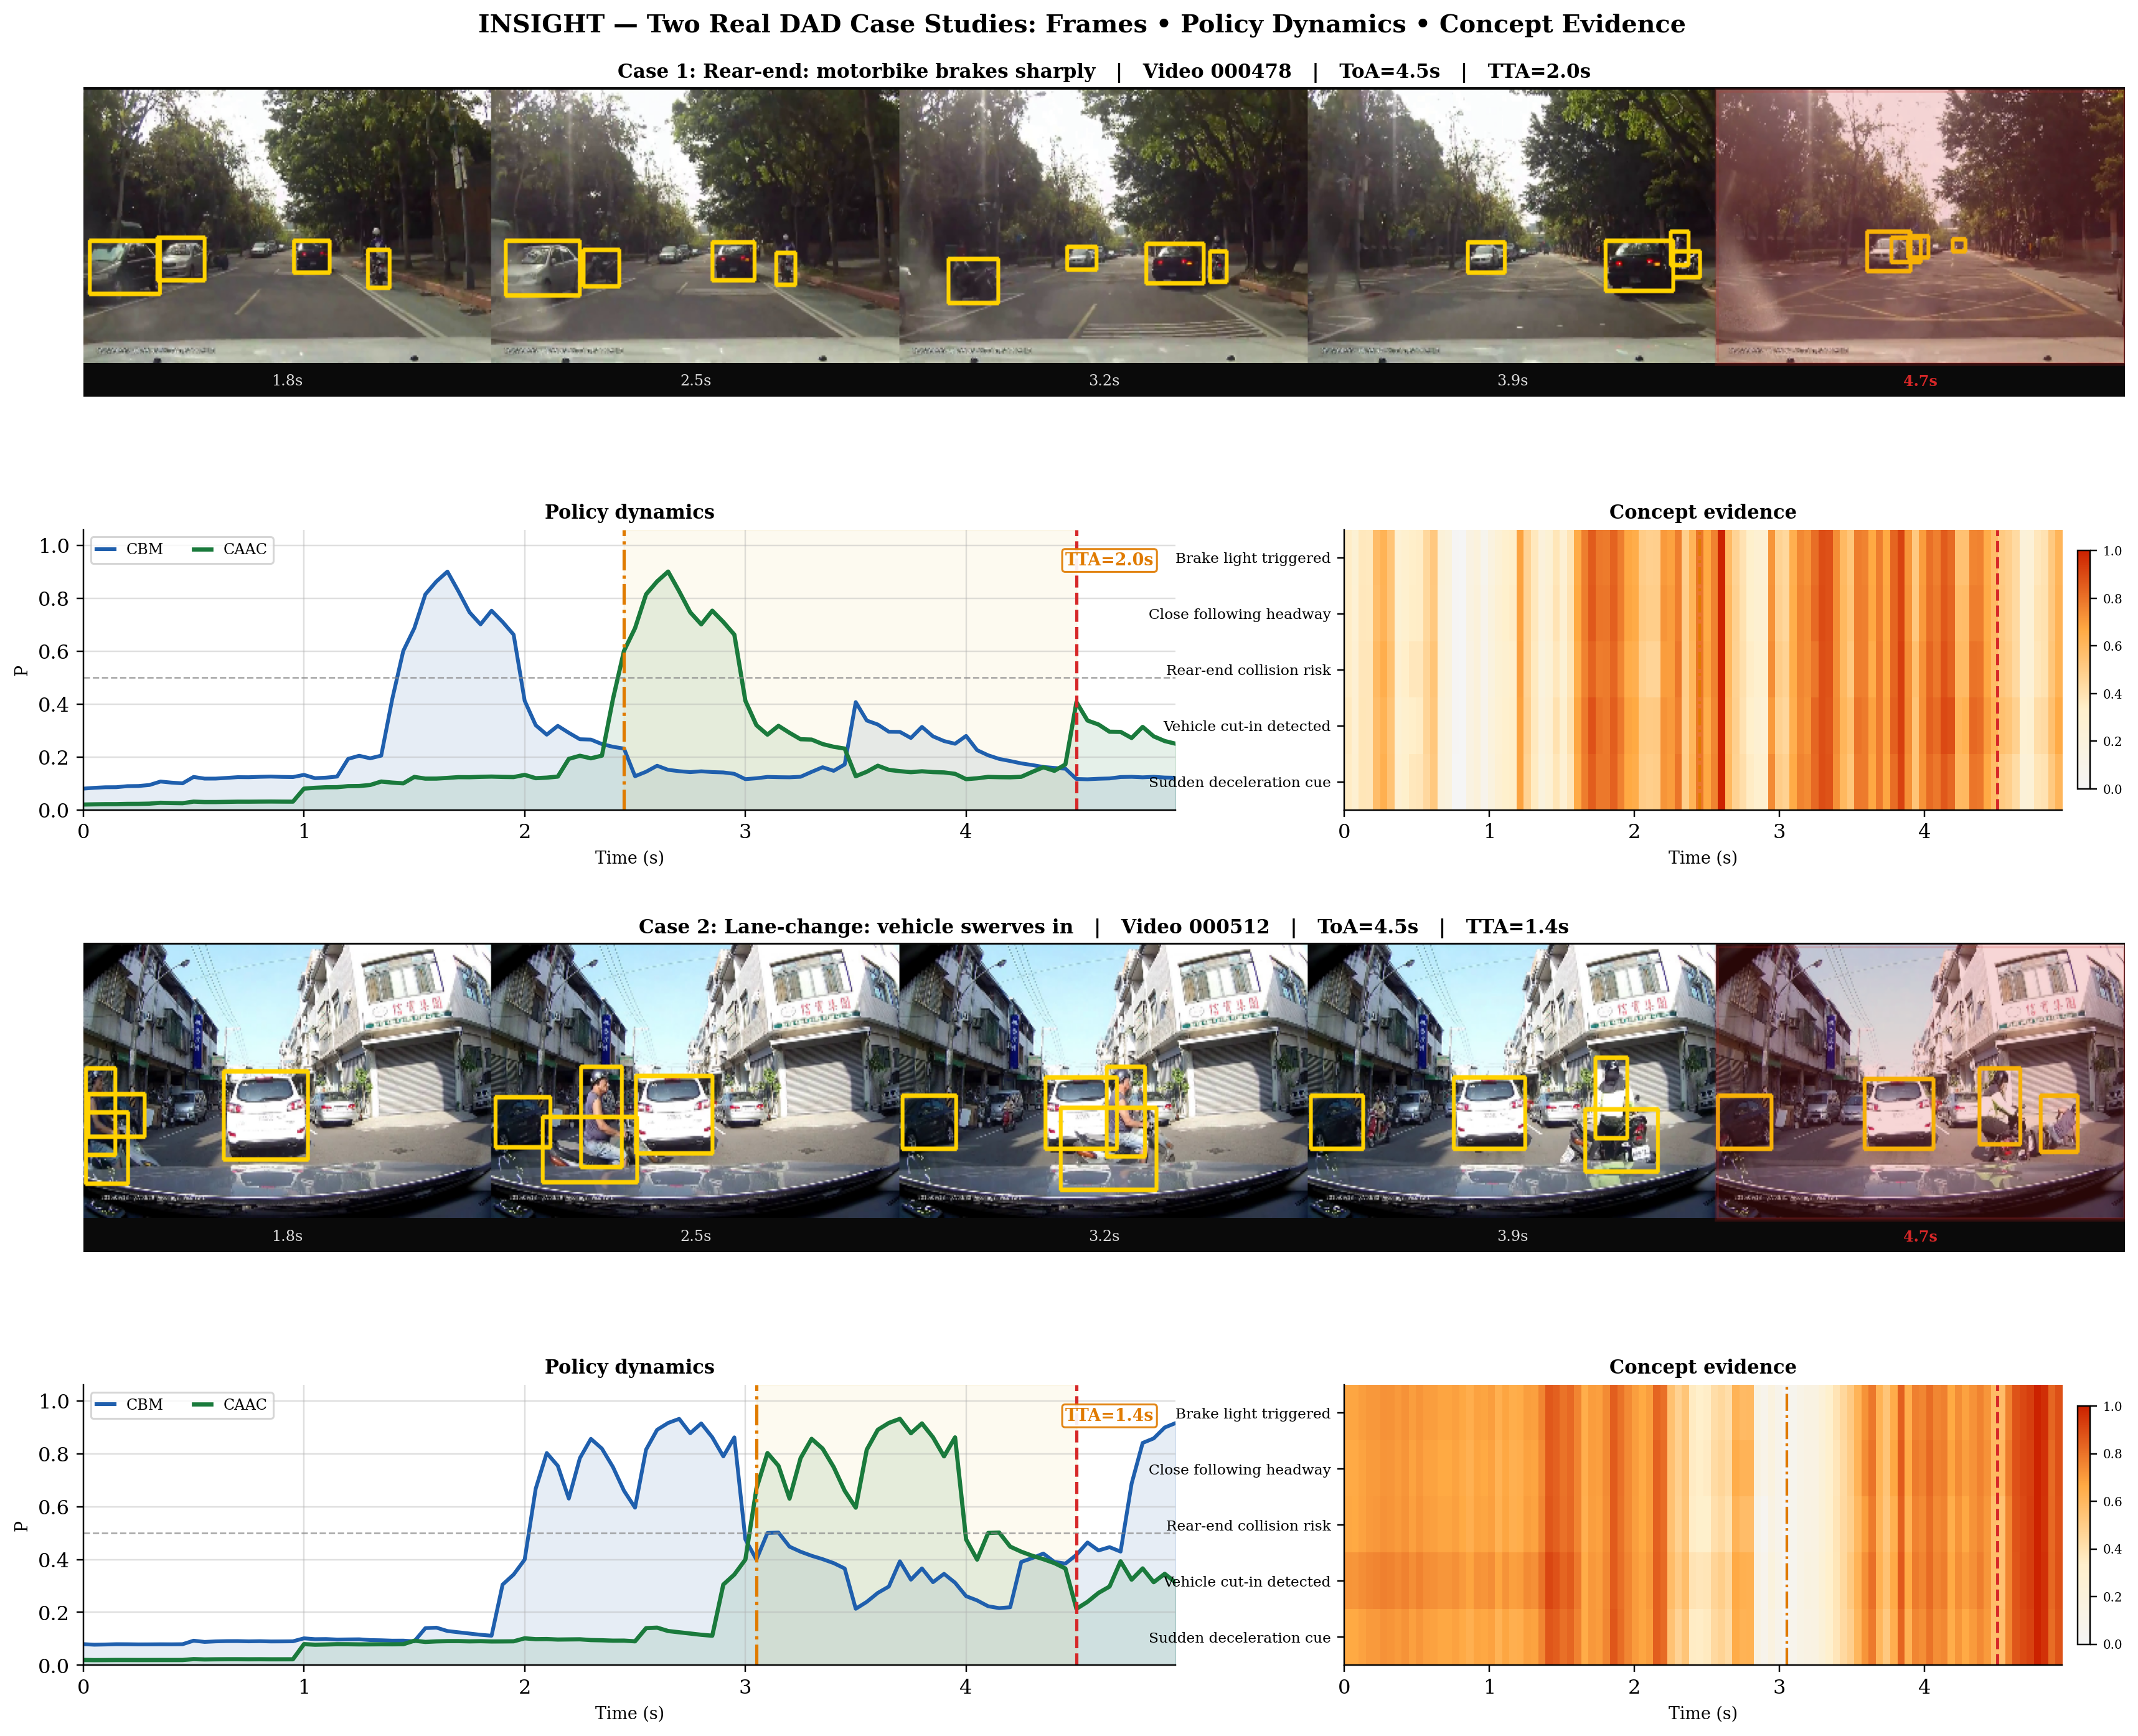
\includegraphics[width=0.98\textwidth]{../figures/insight_fig_appendix_v4_casebank_selected.pdf}
  \caption{\textbf{Selected v4 DAD cases ranked by prediction-branch behaviour.}
  Using the runnable v4 checkpoint, we extract a shortlist containing an
  earlier-warning case, near-threshold borderline cases, and a harder
  low-visibility example. Because the alert surrogate is nearly flat on this
  checkpoint line, the figure should be read as a prediction-level qualitative
  bank rather than as a policy-level alert benchmark.}
  \label{fig:appendix_v4_casebank_selected}
\end{figure*}

\paragraph{Case diversity.}
Across rear-end, lane-change, and intersection scenarios, the dominant
concepts change substantially, but the qualitative pattern stays similar: the
\cbm{} surfaces plausible risk factors first, and the downstream timing signal
responds as those factors rise. The appendix figures also show that visually
strong cases vary in difficulty, from clean agent separation to cluttered or
low-visibility scenes.

\paragraph{Policy-before-peak behaviour.}
In selected qualitative figures, the green \caac{} curve can cross its alert
threshold \emph{before} the blue raw accident-probability curve peaks. This is
consistent with the intended effect of the time-remaining reward: the timing
consumer can respond to a rising semantic trend rather than waiting for maximal
confidence. We present this as qualitative support for the design, not as a
standalone policy benchmark.

\paragraph{Frame--concept alignment.}
The strongest visual evidence occurs when a concrete scene change is mirrored
by a concept change: brake lights activate, headway shrinks, or a vehicle cuts
into the ego lane, and the corresponding concept rows intensify in the
heatmap. Not every high-scoring sample is equally legible, which is why case
selection matters for qualitative presentation.

\subsection{Failure Modes, Robustness Considerations, and Dataset-Specific Discussion}
\label{app:failure}

\paragraph{Low-visibility conditions.}
Night-time and poor-weather scenes remain challenging. In these settings, the
ROI features are weaker and concept activations become less reliable,
especially for fine-grained cues such as brake lights or subtle lane-boundary
signals. The resulting failure mode is usually concept under-activation rather
than an obviously incorrect timing policy.

\paragraph{Crowded scenes.}
When many agents are present simultaneously, the object-focused aggregation
must compress a large amount of interaction structure into a fixed hidden
state. This can dilute the representation of the single most critical risk
agent. A natural next step is a more explicit risk-agent selection mechanism
layered on top of the concept bottleneck.

\paragraph{Concept vocabulary coverage.}
Although 837 concepts provide broad coverage, rare corner cases still exist
where the needed concept is absent or too coarse. This is a limitation of any
finite concept vocabulary. Future work could investigate adaptive or
hierarchical concept sets that retain auditing benefits while improving
long-tail coverage.

\paragraph{Why A3D and DAD behave differently.}
The qualitative evidence suggests that the relative value of semantic
structuring is dataset-dependent. In A3D, many hazards develop progressively,
so early concept growth is especially useful for anticipation. DAD is harsher:
the margin between weak early signal and crash onset is smaller, and the scenes
are often more cluttered. This likely explains why DAD is both a harder
benchmark and a more sensitive test of concept reliability.

\paragraph{Robustness interpretation.}
The main robustness point is that the semantic interface remains useful across
multiple datasets and accident types even when controllability is not uniformly
strong across all checkpoints and scenes. The v4 appendix search therefore
serves as prediction-level qualitative support rather than as a policy-level
ranking result.
accident anticipation should be treated as a concept-conditioned sequential
decision problem, not merely as frame-wise classification with post-hoc
explanation.


\end{document}
